\documentclass[letterpaper,twocolumn,10pt]{article}
\usepackage{usenix,epsfig,endnotes}
\usepackage[utf8]{inputenc}
% \title{Analyzing the Effectiveness of Client-Side Content-Based Anti-Phishing in the Browsers}
% \author{}
% \date{November 2020}

\usepackage{colortbl}
\usepackage{tikz}
\usepackage{amsmath}
\usepackage{filecontents}
\usepackage{cite}
\usepackage[utf8]{inputenc}
\usepackage{amsmath,amssymb,amsfonts}
\usepackage{algorithmic}
\usepackage{pbox}
\usepackage{hyperref}
\usepackage{graphicx}
\usepackage{textcomp}
\usepackage{graphics}
\usepackage{comment}
\usepackage{xcolor}
\usepackage{booktabs}
\usepackage{pgfplots}
\usepackage{pgfplotstable}
\usepackage{rotating}
\usepackage{multirow}
\usepackage{longtable}
\usepackage{lipsum}
\usepackage{adjustbox}
\usepackage{amssymb}% http://ctan.org/pkg/amssymb
\usepackage{pifont}% http://ctan.org/pkg/pifont
\newcommand{\cmark}{\ding{51}}%
\newcommand{\xmark}{\ding{55}}%


% \newcommand{\red}[1]{{\color{red}#1}}
% \definecolor{bblue}{HTML}{4F81BD}
% \definecolor{rred}{HTML}{C0504D}
% \definecolor{ggreen}{HTML}{9BBB59}
% \definecolor{ppurple}{HTML}{9F4C7C}
% \def\BibTeX{{\rm B\kern-.05em{\sc i\kern-.025em b}\kern-.08em
%     T\kern-.1667em\lower.7ex\hbox{E}\kern-.125emX}}
% %

% \usepackage{booktabs} % For formal tables
% \usepackage{epstopdf}
% \usepackage{epsfig}
% \usepackage{multirow}
% \RequirePackage{listings}
% \lstset{%
%   language=C,
%   basicstyle=\small\ttfamily,
%   xleftmargin=0.5cm,
%   numbers=left,
%   numberstyle=\scriptsize,
%   %numberstyle=\tiny\ttfamily
%   stepnumber=1,
%   numbersep=8pt,
%   showstringspaces=false,
%   breaklines=true,
%   frame=lines,
%   tabsize=4,
%   escapeinside={\%*}{*)}, % if you want to add a comment within your code
%   captionpos=b,
%   % morestring=[s]{L}{;},
% }
\usepackage[utf8]{inputenc}

\usepackage[all]{nowidow}

\clubpenalty=10000
\widowpenalty=10000
\brokenpenalty=4991
\predisplaypenalty=10000
\postdisplaypenalty=1549
\displaywidowpenalty=1602

\hyphenation{op-tical net-works semi-conduc-tor}

\usepackage[utf8]{inputenc}
\usepackage[english]{babel}
\usepackage{float}

\begin{document}

\title{\Large \bf Analyzing the Effectiveness of Client-Side Content-Based Anti-Phishing in the Browsers}
	
	%\author{} % end author
	
\maketitle


%\section{Introduction}

%Outline{
%The new version for the introduction part

% %This section will cover the following concepts:

% First paragraph:

% Growing phishing attacks and its damage.

% Second paragraph:

% the growing sophistication of attacks

% Third paragraph:

% the effectiveness of empirical measurements to identify ecosystem gaps:

% Fourth paragraph:

% the increasing importance of such defenses given their ability to be proactive

% sixth paragraph: 



% What we have done in our paper:

% This paper aims to look deeper into the content-based anti-phishing in industrial browsers.%%
%Outline}

%Edited introduction:
\section{Introduction}
Phishing attacks remain popular among criminals with the growth of sophisticated phishing websites as well as the aid of evasion techniques such as cloaking~\cite{oest2020phishtime,internet,hao2013understanding}. With the support of illicit underground services, these fraudulent sites cause collateral damage by harming the reputation of impersonated brands, compromising legitimate infrastructure, and demands effort to assuage abuse~\cite{zhang2007cantina}.

There are two categories of approaches in protecting users against phishing attacks:reactive and proactive methods. Blacklists, as a reactive approach, require blacklists entities to validate the fraudulency of the visited website. Content-based methods as a proactive approach analyze the content of the website~\cite{wang2011verilogo}.

Blacklists have shown high accuracy (low false-positive rates) in identifying phishing websites. However, there is a noticeable window of risk between the time that the phishing site first goes up and the time it is available in the browsers' blacklists. Moreover, Blacklists also not efficient in detecting \textit{targeted phishing attacks} such as \textit{spear phishing}, and \textit{whaling} attacks which target a specific group of people or the important individuals at an organization ~\cite{burns2019spear}. These attacks utilize social engineering to customize the attacks. They occur on a small geographical and timing scale. Thus, the content-based anti-phishing defense method comes to the rescue to not only validate the visited website proactively to identify likely phishing pages but to also detect the small phishing campaign.

Nowadays, the modern desktop and mobile web browsers utilize a content-based anti-phishing system beside the default anti-phishing blacklists to protect the user against known and unknown malicious sites. The primary purpose of appending this mechanism to the browsers is to cover the shortcomings of blacklists in detecting new malicious sites~\cite{googlechromeprivacywhitepaper}. Still, there is a need to evaluate these client-side classifiers to assess their performance, especially when facing phishing attacks with evasion techniques. Moreover, this thorough evaluation will assist in increasing the security of the users in the browsers with the client-side anti-phishing system.

In this paper, we study the effectiveness of the client-side anti-phishing system, including the content-based, Real-time, and password protection mechanism deployed in Chrome, as the most popular browser in the world. We focus on addressing the client-side anti-phishing shortcomings of Google Safe Browsing~(GSB) since it has the largest share of users worldwide, with around three billion active users~\cite{statcounterall}.
For this purpose, we propose an empirical analysis contributing to the Phishfarm framework~\cite{oest2019phishfarm}
%to evaluate content-based anti-phishing functionality and its effectiveness in blacklisting new brand and unseen phishing websites. 
First, we extract the Chrome browsers' built-in classifier, Google's phishing pages filter (GPPF), via the static and dynamic analysis on chromium implementation. 
The extracted classifier information includes the classification algorithm, the number of scoring rules, the corresponding rules weight, scores formula, and the classifier's features. 
Based on classifier information, we evaluate the client-side and server-side classifier. Our experiments reveal that only 12\%  of the phishing websites have scored more than the threshold, and the GSB server only detects 15\%  of the phishing websites among the websites that the client-side classifies as phishing websites. 

The central part of our experiment, done on a large scale, is measuring the content-based anti-phishing effects on the blacklist's speed and coverage.
Nowadays, many phishing kits employ server-side cloaking, and they make the presence of cloaking a  norm within modern phishing websites~\cite{oest2018inside}.
To perform a real-world study, we considered server-side cloaking with an IP address filter as a common evasion technique in desktop and mobile browsers.
We consider four different anti-phishing components that the chrome browser uses: (1) blacklist, (2) Content-based , (3) real-time, and (4) password protection. This browser utilize these anti-phishing mechanisms in three different security layers: (1) no protection, (2) standard Protection, and (3) enhanced protection
%We consider three defense layers of the chrome browser: (1) Blacklist, (2) Content-based anti-phishing, and (3) Real-time anti-phishing.
We perform this experiment for seven days and monitor the blacklisting process to see the effects of Chrome's different defense layers in dealing with cloaking and reporting to the main entities.
The experiment results lead to several interesting findings: 
despite GSB claims, the client-side content-based anti-phishing does not affect the blacklisting speed and accuracy.
%The It has significant bugs and shortcomings in scoring the phishing websites. The uncovered classifier's scoring and algorithm bugs lead to an inefficient content-based anti-phishing system in the real-world. 
Moreover, the chrome browser's real-time anti-phishing system has serious shortcomings, and the server classifier results in the real-time anti-phishing requests are inefficient. 
In terms of privacy, in the client-side anti-phishing ecosystem, after detecting a malicious site, client sends a request to the server to run the server-side classifier and analyze the site. The browser sends some privacy-related information in this request.
The password protection approach is also vulnerable to manipulating DOM elements names. 
There is also a considerable inconsistency in the desktop and mobile blacklists. Even in the absence of cloaking, and after reporting the phishing sites to the blacklists entities, mobile chrome blacklists providers do not blacklist reported phishing sites.

The contributions of our paper are as follows:

\begin{itemize}
    %\item A longitudinal empirical measurement of user security in the client-side content-based anti-phishing ecosystem. 
    \item The first in-depth and continuous long-term measurements of chrome browser's anti-phishing, including content-based, real-time and password protection methods, and disclosure of the weaknesses and inefficiency of these three components.
    %\item The first empirical study of chrome real-time anti-phishing methods and its effect on the blacklisting of un-seen phishing websites.
    \item Identification and disclosure of remaining significant inconsistency in the desktop and mobile blacklists.
    \item The first empirical study to evaluate the GSB server-side classifier performance dealing with phishing websites in the wild.
    \item Disclosure of serious privacy issues in the chrome browser's client-side content-based anti-phishing system
\end{itemize}

% \section{Introduction}

% Although a large-scale ecosystem is employed to protect users, phishing remains popular among criminals with the help of the growth in sophistication of phishing websites, and subsequently cause collateral damage by harming the
% the reputation of impersonated brands, compromising legitimate
% infrastructure, and demand effort to assuage abuse~\cite{zhang2007cantina}.



%  %**the growing sophistication of attacks:
%  Phishing websites continue to be more sophisticated with the aid of evasion techniques like cloaking~\cite{oest2020phishtime}.
%  %Phishing kits have claoking 
%  Due to the support of illicit underground services, phishing is still scalable and has a low entry barrier even for sophisticated and evasive attacks~\cite{internet,hao2013understanding}.
 
% %  , the client-side evasion techniques
% Blacklists are a reactive approach. They require that blacklist providers visit the suspicious site, validate that it is indeed a phishing site, and send this information to the client. 
% Although this approach has low false-positive rates, it leads to a noticeable window of risk between the time that phishing site first goes up and the time it is made available in the browser blacklist~\cite{wang2011verilogo}. 

% On the other hand, content-based anti-phishing approaches are proactive approaches against phishing attacks. This defense method proactively analyzes the content of the site that users intend to visit, evaluates the site's validation,identify likely phishing pages, and protects users against not-blacklisted phishing sites.

% Nowadays, the main desktop and mobile web browsers utilize a content-based anti-phishing system beside the default anti-phishing blacklists to protect the user against known and unknown malicious sites. The primary purpose of appending this mechanism to the browsers is to cover the shortcomings of blacklists in detecting new malicious~\cite{googlechromeprivacywhitepaper}. 

% % Table \ref{tab:Browsers anti-phishing settings} shows the anti-phishing methods deployed in the major web browsers.

% % We focus on Chrome browser in this paper.
% %inja begam chera asan client-side umad
% %second paragraphs: previous works
% % Despite the importance of browser built-in anti-phishing for the users' security, there have been no longitudinal, systematic, real-word studies of the browsers' client-side content-based anti-phishing ecosystem.

% % Despite the importance of the browser built-in anti-phishing for the users' security, no longitudinal, systematic and real-world study has been conducted specifically on the client-side content-based anti-phishing ecosystem of the browsers.
% % Few works have been done in evading the client-side classifier providing effective evasion attacks on ML-based web phishing classifiers~ \cite{lei2020advanced,liang2016cracking}.
% Although prior work has evaluated client-side classifiers~\cite{lei2020advanced,liang2016cracking}, these studies did not assess the client-side's real-world impact classifier performance considering common phishing attacks with evasion techniques. Also, no work has been done on the security of the users in the browsers' content-based anti-phishing system.
% % However, no work has been done on users' security in the browsers' content-based anti-phishing system.
% % However, no work has been done on the security of the users in the browsers' content-based anti-phishing system.
% % On the other hand, although the empirical evaluation is crucial to identify the anti-phishing ecosystem's vulnerabilities, there is no research has been done in empirical measurements of the content-based classification is effective in blacklisting 0-day phishing websites.
% % On the other hand, although the empirical evaluation is crucial in identifying the vulnerabilities of the anti-phishing ecosystem, no research has been done to show the effectiveness of the content-based classification in blacklisting new phishing websites. Protecting users against phishing attacks 
% The growth of new and more sophisticated phishing websites increases the importance of proactive defenses. There are many studies in evaluating the blacklists, but few works have been done in the client-side content-based system as a second defense layer of commercial browsers. 



% %%% **the effectiveness of empirical measurements to identify ecosystem gaps:
% %%%How the client-side browsers work in the real word
   
% %%%**limited studies of client-side browser defenses 


%  %%%**increasing importance of such defenses given their ability to be proactive

% %forth paragraph: in this paper what we have done
% In this paper, we thoroughly evaluate the client-side content-based anti-phishing in chrome, the most popular browser in the world, performing an empirical analysis on this browser.
% We focus on GSB since it has the largest share of users worldwide, with around three billion users. We tried to evaluate chrome anti-phishing power against the phishing attacks to address the GSB client-side anti-phishing shortcomings.

% For this purpose, we propose an empirical analysis contributing to the Phishfarm framework~\cite{oest2019phishfarm} to evaluate content-based anti-phishing functionality and its effectiveness in blacklisting new brand and unseen phishing websites.  First, we extract the Chrome browsers' built-in classifier, Google's phishing pages filter (GPPF) via the static and dynamic analysis on the implementation of chromium. 
% The extracted classifier information includes the classification algorithm, the number of scoring rules, the corresponding rules weight, scores formula, and the classifier's features. 
% Based on classifier information, we evaluate the client-side and server-side classifier. Our experiments reveal that only 12\%  of the phishing websites have scored more than the threshold, and the google safe browsing server only detects 15\%  of the phishing websites.

% % Based on classifier information, we design a framework to perform two preliminary experiments: 
% % 1)Client-side classifier: the results of this experiment show that around 12 percent of the phishing websites have scored more than the threshold.
% % 2)Server-side classifier: this experiment demonstrates that the server's responds show that google safe browsing server only detects 15 percent of the phishing websites.
% % (1) We feed the classifier with 200 phishing sites from the Phishtank database and observe the classifier's results.
% % The results show that around 12 percent of the phishing websites have scored more than the threshold.
% % (2) We modify the client-side classifier threshold to send request to the server for 100 phishing websites to analyze the efficiency of the server-side classifier.
% % The server's responds show that google safe browsing server only detects 15 percent of the phishing websites.
% The main part of our experiment that has been done on a large scale is the measuring of the content-based anti-phishing effects on the blacklist's speed and coverage.
% Nowadays, many phishing kits employ server-side cloaking, and they make the presence of cloaking a  norm within modern phishing websites~\cite{oest2018inside}.
% To perform a real-world study, we considered server-side cloaking with IP address filter as a common evasion technique in the desktop and mobile browsers.
% % In this experiment, we considered cloaking as a main evasion technique in the desktop and mobile browsers. 
% % We consider 14 batches to cover the different combinations of browser settings and implementation of cloaking, and reporting to the blacklist entities in different ways. We assign 35 sites for each group. In May 2020, we created a total of 490 new phishing websites to evaluate content-based anti-phishing in terms of different browser defense layers and cloaking.
% We consider three defense layers of the chrome browser: (1) Blacklist, (2) Content-based anti-phishing, and (3) Real-time anti-phishing.
% We perform this experiment for seven days and monitor the blacklisting process to see the effects of different defense layers of chrome in dealing with cloaking and reporting to the main entities.
% The experiment results lead to several interesting findings: 
% Despite GSB claims, the client-side content-based anti-phishing does not affect the blacklisting speed and accuracy.
% %The It has significant bugs and shortcomings in scoring the phishing websites.The uncovered classifier's scoring and algorithm bugs lead to an inefficient content-based anti-phishing system in the real-world. 
% Moreover, the chrome browser's real-time anti-phishing system has serious shortcomings, and the server classifier results in the real-time anti-phishing requests are inefficient. 
% In terms of privacy, in the client-side anti-phishing ecosystem, after detecting a malicious site client sends a request to the server to run the server-side classifier and analyze the site. The browser sends some privacy-related information in this request.
% The password protection approach is also vulnerable to manipulating DOM elements names. 
% There is also a considerable inconsistency in the desktop and mobile blacklists. Even in the absence of cloaking, and after reporting the phishing sites to the blacklists entities, mobile chrome blacklists providers do not blacklist reported phishing sites.
% % \begin{enumerate}
% %     \item Despite GSB claims, The client-side content-based anti-phishing does not affect the blacklisting speed and  accuracy.
% %     \item The client-side content-based classifier has significant bugs and shortcomings.
% %     \item The real-time anti-phishing system has serious shortcomings, and the server classifier results in the real-time anti-phishing requests are inefficient.
% %     \item In the client-side anti-phishing ecosystem, after detecting a malicious site client sends a request to the server to run the server-side classifier and analyze the site. The browser sends some privacy-related information in this request.
% %     \item There is considerable inconsistency in the desktop and mobile blacklists. Even in the absence of cloaking, and after reporting the phishing sites to the blacklists entities, mobile chrome blacklists providers do not blacklist reported phishing sites.
% % \end{enumerate}

% The contributions of our paper are as follows:

% \begin{itemize}
%     %\item A longitudinal empirical measurement of user security in the client-side content-based anti-phishing ecosystem. 
%     \item The first in-depth and continuous long-term measurements of chrome browser's anti-phishing including content-based, Real-time and password protection methods, and disclosure of the weaknesses and inefficiency of these three components.
%     %\item The first empirical study of chrome real-time anti-phishing methods and its effect on the blacklisting of un-seen phishing websites.
%     \item Identification and disclosure of remaining significant inconsistency in the desktop and mobile blacklists.
%     \item The first empirical study to evaluate the GSB server-side classifier performance dealing with phishing websites in the wild.
%     \item Disclosure of serious privacy issues in the chrome browser's client-side content-based anti-phishing system
% \end{itemize}

% %Moved to the earlier paragraphs in Intro
% % In this paper, we focus on GSB since it has the largest share of users worldwide  with around three billion users. We tried to evaluate chrome anti-phishing power againt the phishing attacks to address the GSB client-side anti-phishing shortcomings .  


\section{Background}
% % outline{
%The layout of this section is going to be as follows:
% The first paragraph:
% Briefly about 1)phishing attacks(done) 2)anti-phishing methods(done)
%  3)Our focus on studying Browsers' Content-based Anti-phishing mechanism (not done)} outline
Phishing is a kind of social engineering attack in which attackers (phishers) try to convince a target to disclose sensitive information to a fraudulent website purporting to be a well-known brand~\cite{dodge2007phishing,holz2009learning,mcgrath2008behind}. Phishers also exploit any circumstance to deploy their campaigns,for instance attackers started to exploit new different situation that Corona virus brought to the world\cite{bitaab2020scampandamic}.
Attackers use the harvested information for their own profits~\cite{sood2013crimeware,aleroud2017phishing}.
These attacks compromise user accounts and identities, and on a larger scale, they also damage the targeted brand reputation and burden massive cost to the targeted companies to deploy an extensive anti-phishing system to protect the brand and consumers~\cite{hong2012state}.

Several anti-phishing solutions have been done in detecting phishing attacks. Blacklists and ML-based methods are two major types of anti-phishing approaches. However, blacklists have a significant shortcoming in detecting 0-day attacks~\cite{oest2019phishfarm}. 
On the other hand, ML-based techniques, beyond being scalable and accurate, they are able to detect newly created phishing websites~\cite{whittaker2010large}.
The ML-based approaches are deployed in industrial browsers such as chrome and Edge to cover the blacklists shortcomings~\cite{safebrowsing,mjcaparas}.

%%%'need to add" Chromium vs chrome:
%Chromium is the open-source project behind the google chrome browser. Although chrome has different functionalities that chromium does not, google safe browsing is the same in both. Therefore, we study the GSB source in chromium, and we deployed the chrome browser in the real-world experiment. Our study released the main shortcoming of safe browsing during chromium source code analysis. These findings affect other Chromium-based browsers like  Edge version 84.
\subsection{Website and Webpage Structure}
A website is formed of webpages for presenting the content to the user. A webpage has multiple elements and a basic structure. These elements are presented in the DOM tree; a hierarchical tree shows the webpage's DOM nodes, including element, text, attribute, and comment codes.
The combination of elements, texts, attributes, and scripts determines a web page's appearance and functionalities. 

\subsection{Phishing attacks}

%%% Outline{ In this subsection, we will discuss phishing attacks in more detail:

% Phishing attacks mechanism

% Sophisticating phishing attacks} outline

Phishing attacks consists of three major stages: In the first phase, attackers create a fake website masquerading it as a trusted website to make it difficult for a user to distinguish that it is a fake site. Phishers can deploy these fake sites without expertise technical knowledge by using the phishing kits. Second, they send messages to various users to convince them to click on the phishing website's link. Phishers use social engineering to deceive users to take the action~\cite{dhamija2006phishing,thomas2013trafficking}. If the victim clicks on the link, he visits the phishing websites and inserts sensitive information. In the last stage, the phishers extract the victim's information from the phishing website and monetizing that information~\cite{gupta2018defending}.

 %Starting pandemic they did not hesitate to take advantage of users' increased usage of the Internet and their reliance on it   \cite{bitaab2020scampandamic}   

% \subsection{Browser-based Anti-Phishing}
% %\subsection{Browser-based phishing detection}
% %%% outline { In this subsection, we will provide details about the major browsers' anti-phishing mechanism.

% % Google Safe Browsing, Microsoft Smart Screen, Safari, Opera

% % We show browser-side anti-phishing settings for all the browsers in a table. }outline
%  Due to browsers' strategic position and scale, they play a significant role in defending users' security against phishing attacks~\cite{ma2009beyond}. Many modern web browsers -like Chrome and Microsoft Edge- provide built-in detection tools to protect users against phishing attacks on desktop and mobile platforms. For most industrial browsers these native anti-phishing tools include two type of protecting layer: (1) Blacklist (2) Client-side heuristic.
%  Table \ref{tab:Browsers anti-phishing settings} shows the anti-phishing methods deployed in the major web browsers.
% %  Table \ref{tab:Browsers anti-phishing settings} shows the anti-phishing mechanism used in the different modern web browsers.
%  The browser-side classifier use the ML-based trained approach to analyze the websites that user visits~\cite{liang2016cracking}. As a result, if the classifier suspects that a website is malicious the browser shows ``perminanty" warning page to the user .
%  However, Google Safe Browsing introduced another anti-phishing mechanism called ``Real-Time". When user visits a website, chrome checks the URL against the local lists of thousands of trusted websites. If the URL does not match on the local  white-list, chrome checks the URL with google to evaluate the website's phishy-ness~\cite{googlechromeprivacywhitepaper}. Table \ref{tab: Chrome Security levels} shows chrome browser's anti-phishing layers.
%  Chrome provides Three different levels of security: (1) No protection, (2) Standard Protection, and (3) Advanced Protection.

% %  Chrome provides Three different levels of security: 
% %  1-No protection
% %  2-Standard Protection
% %  3-Advanced Protection
% In this work, we investigate the protection level of these three layers along with their security policies.
% %  In this work, we figure out how these layers protect users and what security policies they provide.

\subsection{Blacklists}

As an access control-based mechanism, blacklists are the first defense layer of the browsers against phishing attacks which is by default enabled in the all the major web browsers (i.e., Chrome, Firefox, Opera, Edge, and Safari), both in desktop and mobile platforms.
When users, even without knowledge about malicious websites, visit a fake site without having third-party security defense software, anti-phishing blacklists protect users by displaying prominent warnings in place of the malicious content.Blacklists were the first large-scale anti-phishing defense deployed in browsers. 
Researchers have proved that blacklists have a significant effect on shutting the phishing campaign down~\cite{sheng2009empirical}.
However, they have noticeable shortcomings, as revealed in the previous studies~\cite{oest2020sunrise}.

Although Google incorporated real-time lookups for phishing URLs and improved the speed of GSB suffer from "up to 30 minutes", this feature is not enabled by default, and it still suffers from the delay of caching and periodically updating the local copy of the URL blacklist database providing the attackers an opportunity to launch their phishing campaign. This change also applies to the mobile version of Chrome. We also evaluated this new feature in our experiments~\cite{google-online-security-blog-2019}. Due to short lifetime of the phishing sites, a few hour of latency can affect the blacklist performance in a significant way, and relying on blacklisting can grow the risk disclosure of all internet users subject to a malicious attack~\cite{oest2020sunrise,sheng2009empirical}.


% Unfortunately, blacklists suffer from reactive approaches' weaknesses as latency and 30 minutes updating windows delay, providing the attackers an opportunity to launch their phishing campaign. 

% The average lifetime of the phishing sites is about three days ~\cite{oest2020sunrise}, and most of them last less than a day; therefore, a few hours of latency can affect the blacklist performance in a significant way. On the other hand, in the term of updating window, relying on blacklisting can grow the risk disclosure of all internet users subject to a malicious attack~\cite{sheng2009empirical}.

However, the effectiveness of this mechanism relies on the coverage, speed, and accuracy~\cite{sheng2009empirical}. Modern web browsers' blacklists utilize different blacklist entities with related characteristics~\cite{bell2020analysis}. For example, one specific phishing site could be blacklisted for the chrome browser's users but not for Edge browser's users.
Even for the browsers that are protected with one blacklist provider entity, although the coverage of the blacklists is the same, the speed of the blacklisting might be different, relying on different implementations in the browsers~\cite{oest2019phishfarm}.
Figure 2 shows the anti-phishing mechanism in the modern web browsers. 
% Unfortunately, blacklists suffer from latency and 30 minutes updating windows delay, providing the attackers an opportunity to launch their phishing campaign. The average lifetime of the phishing sites is about three days ~\cite{oest2020sunrise}, and most of them last less than a day; therefore, a few hours of latency can affect the blacklist performance in a significant way. On the other hand, in the term of updating window, relying on blacklisting can grow the risk disclosure of all internet users subject to a malicious attack~\cite{sheng2009empirical}.

% might be something related to our work: like in this work blah blah related to blacklist: maybe:
We evaluate content-based anti-phishing performance and its effects on blacklisting coverage and speed in chrome browser.

\subsection{Evasion methods}
%%% outline { We elaborate evasion methods here as: 
% How do the evasion method works?
% What are the main evasion methods?
Evasion methods differ in various contexts. In this study we refer to two types of evasion methods:
1)ML-based classifier evasion methods: The purpose of these attacks is to evade classifiers by crafting adversarial samples using various mechanisms even in the black-box scenario without any knowledge about the Model~\cite{anderson2019adversarial}. 
2)Blacklisting Evasion methods : These evasion techniques refer to the various methods used by attackers to avoid being analyzed by security infrastructures~\cite{egele2008survey}.
Phishing sites utilize evasion techniques to avoid revealing malicious content to search engine crawlers while keeping it visible to the potential victims ~\cite{samarasinghe2020cloaking, invernizzi2016cloak,panum2020towards}. 

Attackers increase their return-on-investment(ROI) by deploying evasion methods to delay or prevent blacklisting~\cite{han2016phisheye,nero2011phishing,oest2019phishfarm}. 

Blacklist and heuristic anti-phishing methods are vulnerable to evasion techniques because they depend on content verification and can prevent or make delay in blacklisting~\cite{oest2019phishfarm}.

Previous works have studied evasion techniques like cloaking, redirection, using URL shorteners and code obfuscation~\cite{fette2007learning,cova2008there,chhabra2011phi}.

Cloaking is a well-known evasion technique that attempts to show different content to users than to blacklist infrastructure. When a crawler wants to visit the phishing websites with cloaking, it shows a benign page or an error message~\cite{invernizzi2016cloak}.
% The last paragraph mentions that we evaluate content-based anti-phishing against the cloaking evasion method. %%%}outline 
To the best of our knowledge, it is the first work in evaluating impact of of cloaking on the client-side content-based anti-phishing ecosystem.

\subsection{Ml-based Anti-phishing}

%%% outline { We mainly focus on the chrome anti-phishing system, and it is an ML-based anti-phishing approach. So we discuss more the ML-based anti-phishing methods here.} outline
Machine Learning (ML)-based anti-phishing solutions extract features of the websites and feed this features into a trained model with related rules and weight to phishing detection. However, studies have shown that ML-based classifiers are open to attack to the evasion tricks~\cite{lei2020advanced,laskov2014practical,chen2018automated,xuposter,hu2017black,anderson2019adversarial,aleroud2020bypassing,sabir2020evasion}. 
%difference between ml-based evasion methods and crawler evasion methods

Evasion attacks are effective on practical ML-based classifiers, and at the same time these attacks can be successfully launched without changing the functionalities and appearance~\cite{lei2020advanced}.

As shown in the table~\ref{tab:Browsers anti-phishing settings} most major browsers(e.g. Chrome, Firefox and Edge) implement ML-based anti-phishing in the browser-side to analyze the sites that users seek to visit to detect malicious websites and protect them against them~\cite{mjcaparas,whittaker2010large}.


% % \subsection{Server-Side vs. Client-Side Detection}

\section{Browser-based Anti-Phishing}

Due to browsers' strategic position and scale, they play a significant role in defending users' security against phishing attacks~\cite{ma2009beyond}. Many modern web browsers -like Chrome and Microsoft Edge- provide built-in detection tools to protect users against phishing attacks on desktop and mobile platforms. For most industrial browsers these native anti-phishing tools include two type of protecting layer: (1) Blacklist(reactive) (2) Client-side heuristic(proactive.
Table \ref{tab:Browsers anti-phishing settings} shows the anti-phishing methods deployed in the major web browsers.
%  Table \ref{tab:Browsers anti-phishing settings} shows the anti-phishing mechanism used in the different modern web browsers.
The browser-side classifier use the ML-based trained approach to analyze the websites that user visits~\cite{liang2016cracking}. As a result, if the classifier suspects that a website is malicious the browser shows warning page to the user.
Anti-phishing blacklists that are natively implemented in modern web browsers are managed by different service providers. Google Safe Browsing (GSB) maintains blacklists for Chrome, Safari, Firefox, and Chromium~\cite{safebrowsing}.
By global browser market share as of December 2020, GSB is the most affecting blacklist as it protects approximately 80.60\%  of desktop users and 89.82\%  of mobile users~\cite{statcounterall,browsermarketshare}. We perform our empirical study on chrome browser due to the fact that Google Chrome accounted for 70.33\%  of overall desktop web browser, and 63.28\%  of mobile web browser market share in the world. We focus on evaluating the content-based anti-phishing mechanisim for chrome browser to address this system shortcomings to protect around 3 billion users worldwide~\cite{statcounterdesktop,statcountermobile}.
However, Google Safe Browsing introduced another anti-phishing mechanism called ``Real-Time". When user visits a website, chrome checks the URL against the local lists of thousands of trusted websites. If the URL does not match on the local whitelist, chrome checks the URL with google to evaluate the website's phishy-ness~\cite{googlechromeprivacywhitepaper}. Chrome also is the only browser that warns users when accessing sites with provides an additional ``look-alike URL"~\cite{cimpanu_2019}.
Table \ref{tab: Chrome Security levels} shows chrome browser's anti-phishing layers.
Chrome provides Three different levels of security: (1) No protection, (2) Standard Protection, and (3) Advanced Protection.

%  Chrome provides Three different levels of security: 
%  1-No protection
%  2-Standard Protection
%  3-Advanced Protection
In this work, we investigate the protection level of these three layers along with their security policies.
%  In this work, we figure out how these layers protect users and what security policies they provide.
Standard protection is the default setting for the chrome browser.
%Our user experience study shows that among 115 students, just 4 of them check the security settings and change the default setting to advanced protection.
\begin{table}[]
\centering
\begin{tabular}{p{3.58cm}cccc} 
\hline
\toprule
\small{Security Level}                & \rotatebox[origin=c]{90}{\centering\small{Blacklist}} & \rotatebox[origin=c]{90}{\centering\small\pbox{2cm}{Content-based\\ Anti-phishing}} & \rotatebox[origin=c]{90}{\centering\small\pbox{2cm}{Password-\\protection}} &
\rotatebox[origin=c]{90}{\centering\small\pbox{2cm}{Real-time \\Anti-phishing}}
  \\ 
\hline
\small{No Protection}                 & \cmark         & \xmark                           & \xmark                   & \xmark                        \\
\small{Standard Protection} \footnotesize{(Default)} & \cmark         & \cmark                           & \cmark                   & \xmark                        \\
\small{Advanced Protection}           & \cmark         & \cmark                           & \cmark                   & \cmark                        \\
\bottomrule
\end{tabular}
\caption{Chrome security levels}
\label{tab: Chrome Security levels}
\end{table}
 
\begin{table}
\centering
\begin{tabular}{cccccc} 
\hline
\toprule
\multirow{2}{*}{\small{Browser}} & \multirow{2}{*}{\small{API}} & \multicolumn{3}{c}{\small{Anti-phishing Methods}}            & \multirow{2}{*}{\begin{tabular}[c]{@{}l@{}}\small{Default} \\\small{Enabled} \\\small{Settings} \end{tabular}}  \\ 
\cline{3-5}
                         &                      & \rotatebox[origin=c]{90}{\small\pbox{3cm}{Blacklist\\ \centering(BL)}} & \rotatebox[origin=c]{90}{\small\pbox{3cm}{Content-\\based\\\centering{ (CB)}}} & \rotatebox[origin=c]{90}{\small\pbox{3cm}{Real-time\\ \centering(RT)}} &                                                                                         \\ 
\hline
\small{Chrome}                   & \multirow{3}{*}{\small{GSB}} & \cmark              & \cmark                  & \cmark              & \small{BL,CB}                                                                                      \\
\small{Firefox}                  &                      & \cmark              & \cmark                  & \xmark              & \small{BL, CB}                                                                                  \\
\small{Safari}                   &                      & \cmark              & \xmark                  & \xmark              & \small{BL}                                                                                      \\
\cline{1-2}\small{Edge}                     & \multirow{2}{*}{\small{MSS}} & \cmark              & \cmark                  & \xmark              & \small{BL, CB}                                                                                  \\
\small{IE}                       &                      & \cmark              & \cmark                  & \xmark              & \small{BL, CB}                                                                                  \\
\cline{1-2}
\small{Opera}                    & \small{Opera}                & \cmark              & \cmark                  & \xmark              & \small{BL}                                                                                      \\
\bottomrule
\end{tabular}
\caption{The modern browsers anti-phishing mechanism}
\label{tab:Browsers anti-phishing settings}
\end{table}
 
 
%%%%%%%%%%%%%%%%%%%%%%%% Figure 1
 
%  \begin{figure}
% \centering
% 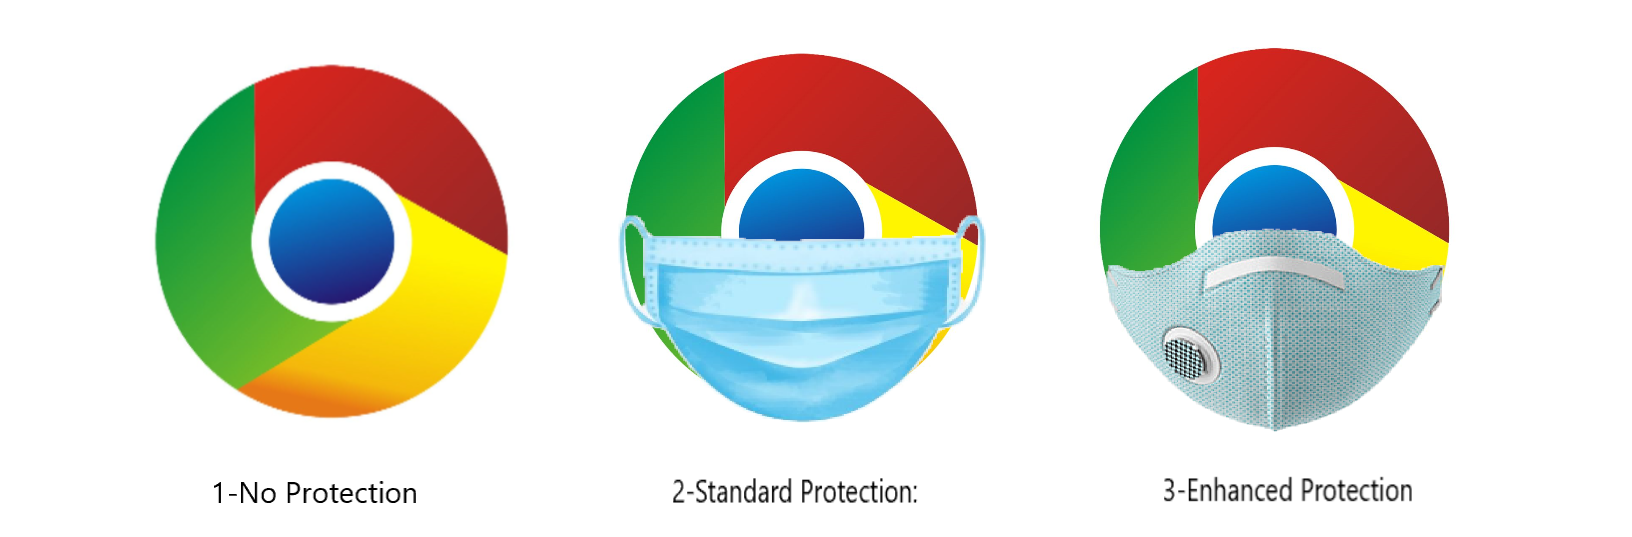
\includegraphics[height=1in, width=3in]{Google.png}
% \caption{Chrome Anti-Phishing Layers}
% \label{fig:phish}
% \end{figure} 
\section{Experimental Methodology}

%% %Outline}

% The layout of this section is going to be as follows:

% In the first paragraph, we state:

% our primary research goals: to evaluate client-side content-based anti-phishing mechanism and its role on the occurrence and timeliness of blacklisting of phishing sites within the industrial browsers

% Express our research questions and what we are going to do and why:

% We illustrate the GSB content-based classifiers Structure on a technical level.

% 1) How does GSB content-based classifier work?

% 2) what attributes does the content-based classifier use in different circumstances?

% 3)What is the relative weight of the different attributes?

% 4)What is the threshold for a page to be classified as phishing?

% 5)what is the server's response to the client, and what are the possible outcomes of the user's request

% 6) [Ultimate goal/research question] How can the GSB classifier be evaded; what are its practical shortcomings in the modern anti-phishing ecosystem?

% 7)Are there any privacy implications associated with the current GSB implementation?
%%outline} 
Our primary research goal is to evaluate the client-side content-based anti-phishing mechanism and its role in the appearance of warnings shown to the user, including occurrence and timeliness of blacklisting phishing sites within Google Chrome browsers.

On a technical level, in addition to blacklist, major browsers conduct client-side ML-based anti-phishing to evaluate the site to determine if it looks malicious site according to the site features. Based on the classifier threshold, browsers send malicious sites, the client-side classifier results and the website's features to the server to evaluate whether the website is a phishing website~\cite{google-online-security-blog-2019}.

Prior studies of browser-based anti-phishing have focused on the blacklist~\cite{oest2019phishfarm,han2016phisheye,sheng2009empirical}, and the few pieces of research have done in the evasion client-side classifier model. However, these works did not consider users' security in the browsers' content-based anti-phishing system. They also did not evaluate the content-based anti-phishing on blacklisting ratio considering cloaking as a popular evasion method. We perform a comprehensive experiment to satisfy these shortcomings. Figure \ref{ frame work} demonstrates the whole framework we deployed in this paper.
\begin{figure*}[h]
  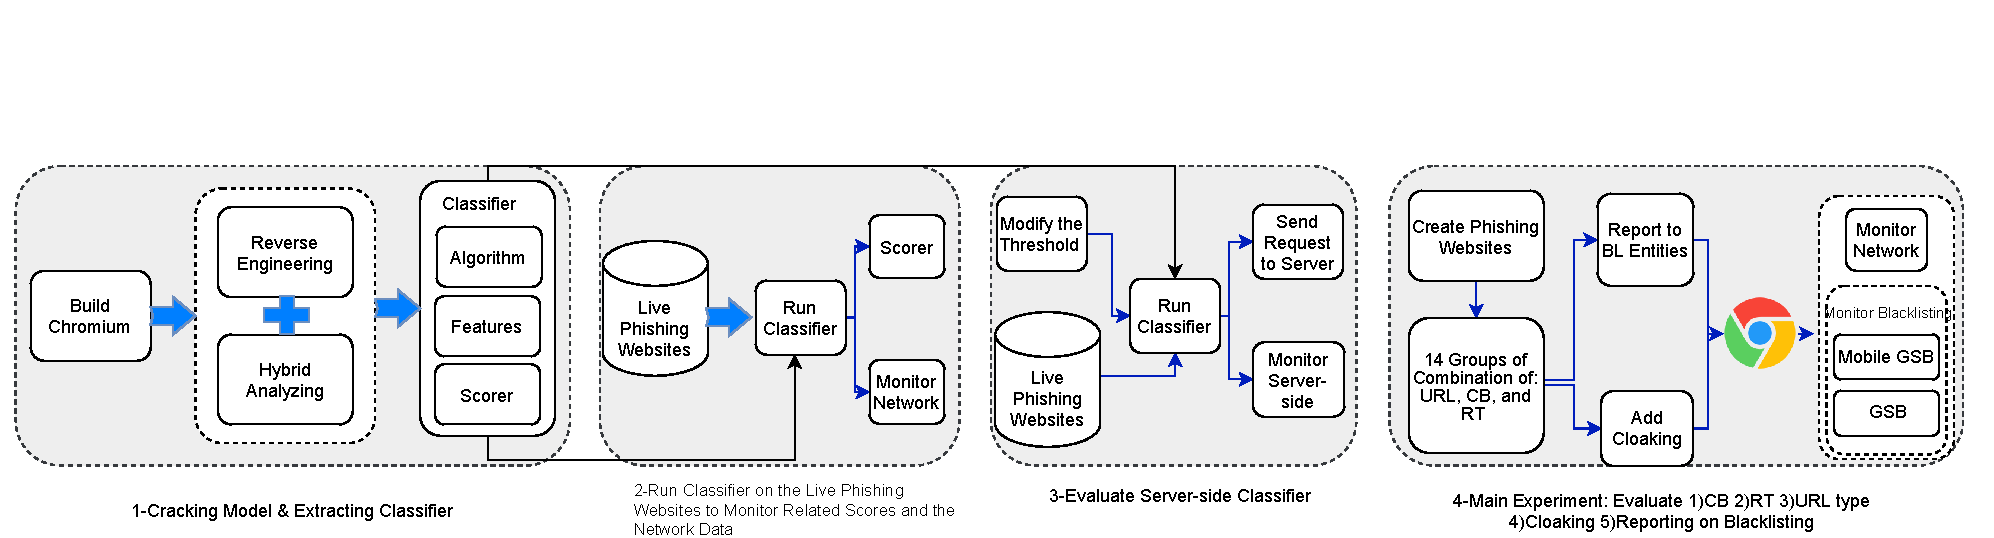
\includegraphics[width=\textwidth,height=6cm]{Untitled Diagram (3).pdf}
  \caption{ Client-side Content-based Anti-phishing Analyzing}
  \label{ frame work}
\end{figure*}

\subsection{Overview}

%%% outline { In this subsection, we discuss the experiment in more details:

% 1)We divide our experiment into two parts:

% a)initial experiment: with live phishing websites from the Phishtank

%     What we do in the initial experiment
    
%     Which and how many websites we use for our experiment
    

% b)main experiment( with our phishing websites and using the Phishfarm framework

%   What we do in the initial experiment
   
%   The Clustering of these websites into 14 batches and each batch's setting ( we show different batches' setting in a table)
   
%   Which and how many websites we use for our experiment

% Main experiment steps:

% 1)Selecting a specific group of anti-phishing entities to test

% 2)Selecting two major web browsers to deploy the experiment on( Chrome browser and Edge)

% 3)Deploying three Virtual Machines (for three different settings of chrome browser) for running the experiment and implement experiment infrastructure on all of them

% 4)Creating 490 new, unique, and previously-unseen PayPal phishing sites with desired cloaking techniques

% 5)Deploying a network traffic capture tool on each Virtual Machine

% 6)Dividing all the websites into 14 groups with different browser settings, reporting, and cloaking

% 7)Reporting five groups of the websites to the entities} outline 


%% We run the experiment for seven days. When the experiment is finished we measure the blacklisting time (the time between reporting and blacklisting ) from the log file. We also have the blacklisting result for all the websites.%%
%Outline





%Our primary research goal is to evaluate GSB content-based classifiers and show what role it plays in the appearance of blacklist warning. 
% %Our primary research goal is to evaluate the client-side content-based anti-phishing mechanism and its role in the occurrence and timeliness of blacklisting of phishing sites within the industrial browsers. 
% For this goal, we illustrate the GSB content-based classifiers Structure on a technical level. How it works, and what attributes does the content-based classifier use in different circumstances. What is the relative weight of the different attributes? What is the threshold for a page to be classified as phishing? What data is sent back to the GSB server, what is the server's response to the client, and what are the possible outcomes on the user's request. [Ultimate goal/research question] How can the GSB classifier be evaded; what are its practical shortcomings in the modern anti-phishing ecosystem?. Are there any privacy implications associated with the current GSB implementation? 


%% \subsection{Overview}
% To perform an effective evaluation of client-side content-based anti-phishing, we deploy a large batch of phishing websites, using different browser settings combined with evasion methods and reporting some of these groups directly to blacklists, then monitor all the websites to see blacklisting coverage and timeliness. Meanwhile, we monitor network traffic to analyze the user's privacy in this ecosystem.  

% On the other hand, to empirically evaluate the server-side anti-phishing classifier's performance, we use a large group of live phishing websites from PhishTank and feed the server-side classifier with these phishing websites and monitor the server responses.
% َAt the high level, we deploy our phishing websites on a large scale. We use 490 different phishing websites divided into 14 batches and direct observations of blacklisting across these different batches for the Google Safe browsing experiment.

% Each batch has a different set of settings of the chrome browser. We further other batches with different types of cloaking. 
% For five batches, once the sites are live, we report their URLs to the anti-phishing entities being tested. We then monitor the entity's response and record the crawling logs, including the time of entities' and blacklist API's visit and blacklisting. We collect network data for each website, meanwhile. 

% In our experiment, we used the phishing sites that all spoofed the Paypal.com login page with permission from PayPal, Inc. All the phishing sites that we used each used new, unique, and previously-unseen .com domain names. We measure the time between our report and browser blacklisting for each site and for doing the experiment more reliably; we did not use any domain more than once.  

% In this work, we deploy a comprehensive study on google client-side anti-phishing mechanism. To study all aspects of the client-side anti-phishing ecosystem we design a multi-layer experiment framework.

We dig into the content-based anti-phishing classifier, the machine learning model, the model's changes, real-time anti-phishing, password protection component ~\cite{google-online-security-blog-2019}, all the anti-phishing tools' effect on the blacklisting speed and coverage, and users' privacy in this system.
% Our experiment are divided to four sections:
Our experiment are divided to two main sections:
\begin{enumerate}
    \item Classifier experiment: 
    \begin{enumerate}
        \item Evaluating Classifier algorithm and scoring results
        \item Evaluating new client-side machine learning model compared to the old model
    \end{enumerate}
    \item Blacklist Experiment:
    \begin{enumerate}
        \item Client-side anti-phishing mechanisms' effects on blacklisting
        \item Analyzing user privacy in the client-side anti-phishing ecosystem
    \end{enumerate}
    % \item Blacklisting experiment
    % \item Analyzing user privacy in the client-side anti-phishing ecosystem
\end{enumerate}

% \begin{enumerate}
%     \item Classifier experiment 
%     \item Evaluating new client-side machine learning model compared to the old model
%     \item Blacklisting experiment
%     \item Analyzing user privacy in the client-side anti-phishing ecosystem
% \end{enumerate}




\subsubsection{Classifier experiment}
\textbf{To evaluate classifier algorithm and scoring results:}
% In this experiment 
we extract the whole client-side anti-phishing complex, including classifier's algorithm, features and the phishy-ness score calculating formula. For this part of the experiment, we repeated steps 1-3 from experiment 2.
% \begin{enumerate}
%     \item Build the chromium source code
%     \item Implement Visual Studio's built-in debugger and network monitoring tools
%     \item Hybrid reverse engineering, including static and dynamic analysis, debugging and logging, and network interpretation, extracts the client-side content-based anti-phishing Classifier
% \end{enumerate}
We have performed this analysis on 100 live phishing sites to extract complete knowledge about the client-side content-based anti-phishing ecosystem. 

% \subsubsection{Evaluating new client-side machine learning model compared to the old model}
\textbf{Evaluating new client-side machine learning model compared to the old mode}:
% On September 2020 in the middle of our study we realized noticeable change in the scorer results. This change appears when we build chromium source code on a new computer to run new classifier evaluation experiment. Deploying reverse engeeniering on the new source code we found the source of these mutation in the scorer results.We realized the client-side anti-phishing model and classifier algorithim have changed, then we decided to add new experiment to our work to evaluate the new released client-side machine learning model and find out this new changes effects on the whole client-side content-based anti-phishing system.  
In September 2020, we realized a noticeable change in the scorer results in the middle of our study. This change appears when we build the chromium source code on a new computer to run a new classifier evaluation experiment.
Chromium is the open-source project behind the google chrome browser. Although chrome has different functionalities that chromium does not, google safe browsing is the same in both. Therefore, we study the GSB source code in chromium, and we deployed the chrome browser in the real-world experiment. Our study released the main shortcoming of safe browsing during chromium source code analysis. These findings affect other Chromium-based browsers like  Edge version 84.
Deploying reverse engineering on the new source code, we found the source of this mutation in the scorer results. We realized the client-side anti-phishing model and classifier algorithm have changed. Then we decided to add a new experiment to our work to evaluate the newly released client-side machine learning model and find out the effects of this new change on the whole client-side content-based anti-phishing system. 

We considered two factors in comparison to the results of the classifier on old and new phishing websites:
\begin{enumerate}[label=(\alph*)]
    \item Improvement of the client-side machine learning model
    \item The improvement of the phishers knowledge about defeating the client-side classifier( The advancement of the URL and content of the phishing websites to misclassify by the client-side machine learning model)
\end{enumerate}
%a-	Improvement of the client-side machine learning model

%b-	The improvement of the phishers knowledge about defeating the client-side classifier( The advancement of the URL and content of the phishing websites to misclassify by the client-side machine learning model)

This experiment is described in the following steps:
\begin{enumerate}
    \item We repeated steps 1-3 from experiment 2.
    \item We collected phishing websites for earlier years.
\end{enumerate}

To perform an accurate comparison between the new and old models, we consider that the growth in sophistication of recent phishing attacks may weaken the classifier's results with the new model. Therefore, we run two models on old and new phishing websites.
Since phishing websites' lifetime is not long, we could not access old phishing websites using their URLs.For this purpose, we used the KitPhisher tool~\cite{cybercdh} to obtain phish kits for 2016 and redeploy the phishing websites for 2016.
Phish kits are a unified set of tools that phishers use to deploy a phishing site on a server~\cite{mccalley2011analysis}. The study conducted in 2018~\cite{oest2018inside} showed that the phishing kits started to provide different types of cloaking to make the phishing attacks more sophisticated. To provide phish kits without these techniques, we used phish kits of two years earlier than the time that this study has implemented.


\subsubsection{Blacklisting experiment}
In this section, we discuss three metrics that we consider to evaluate blacklists. We also explain the experiment structure as well as the specific blacklist that we use in our study. 

The blacklist performance metrics are described in table~\ref{tab:Blacklisting metrics}. We consider blacklist's ability to discover new suspected URLs
(\textit{Discovery})as one performance parameter, and blacklist's ability to blacklisting discovered URLs (\textit{Detection})  as another performance metric. To evaluate detection parameter we use two sub-metrics: \textit{Coverage} and \textit{Speed}~\cite{oest2020phishtime} that also are briefly explained in table~\ref{tab:Blacklisting metrics}. 
% . GSB is the most affecting blacklist since it supports approximately 80.30\% of desktop users and 92.22\%  of mobile users~\cite{safebrowsing}.
We focus our study on GSB due to its large potential impact. However, our methodology and framework could be applied to evaluate other blacklist providers such as \textit{Microsoft SmartScreen}, \textit{Opera’s fraud and malware protection}, and other alternatives.

To perform an effective evaluation of client-side content-based anti-phishing, we deploy a large batch of phishing websites, using different browser settings combined with evasion methods and reporting some of these groups directly to blacklists, then monitor all the websites to see blacklisting coverage and timeliness. Meanwhile, we monitor network traffic to analyze the user's privacy in this ecosystem and understand the browser's interactions at the GSB backend.
% Please add the following required packages to your document preamble:
% \usepackage{multirow}
% \usepackage{graphicx}
% \usepackage{multirow}


\begin{table}
\centering
\scalebox{0.93}{
\begin{tabular}{lll} 
\hline
\toprule
\multicolumn{2}{l}{\begin{tabular}[c]{@{}l@{}}BL Performance\\ Metrics \end{tabular}} & Description                                                                                                                     \\ 
\hline
\multicolumn{2}{l}{Discovery}                                                         & \begin{tabular}[c]{@{}l@{}}\small{Blacklist’s ability to identify}\\\small{new suspected URLs}\end{tabular}                                      \\
\hline
\multirow{2}{*}{Detection} & Coverage                                                 & \begin{tabular}[c]{@{}l@{}}\small{The proportion of the discovered}\\ \small{URLs that are correctly blacklisted\\ at any point} \end{tabular}  \\ 
\cline{2-3}
                           & Speed                                                    & \begin{tabular}[c]{@{}l@{}}\small{The time delay between} \\\small{discovery and blacklisting} \end{tabular}                                    \\

\bottomrule
\end{tabular}}
\caption{Blacklisting evaluation metrics~\cite{oest2020phishtime}}
\label{tab:Blacklisting metrics}
\end{table}

On the other hand, to empirically evaluate the server-side anti-phishing classifier's performance, we use a large group of live phishing websites from PhishTank and send them to the server-side classifier with and monitor the server responses.
At a high level,We deploy our phishing websites on a large scale. 
%To cover all the parameter study we needed 14 batches. we consider 35 website for each batches to have good study
We consider 14 batches to cover the different combinations of browser settings and implementation of cloaking, and reporting to the blacklist entities in different ways. We assign 35 sites for each group. In May 2020, we created a total of 490 new phishing websites to evaluate content-based anti-phishing in terms of different browser defense layers and cloaking.We performed direct observations of blacklisting across these different batches for the Google Safe browsing experiment. 
% We use 490 different phishing websites divided into 14 batches and direct observations of blacklisting across these different batches for the Google Safe browsing experiment.
% Each batch has a different set of settings of the chrome browser. We further other batches with different types of cloaking. 

For five batches, once the sites are live, we report their URLs to the anti-phishing entities being tested. We then monitor the entity's response and record the crawling logs, including the time of entities' and blacklist API's visit and blacklisting. Meanwhile, we collect network data for each website.

In our experiments, we used the phishing sites that all spoofed the Paypal.com login page with permission from PayPal, Inc. All the phishing sites that we used each used new, unique, and previously-unseen .com domain names. We measure the time between our report and browser blacklisting for each site and for doing the experiment more reliably; we did not use any domain more than once.  
This experiment steps are described below:  

% Blacklisting experiment:

\begin{enumerate}
    \item Selecting a specific group of anti-phishing entities to test
    \item Configuring Chrome browser to deploying experiment on, Deploying three Virtual Machines (for three different settings of chrome browser) for running the experiment and implement experiment infrastructure on all of them, and Deploying a network traffic capture tool on each Virtual Machine
    \item Creating 490 new, unique, and previously-unseen PayPal phishing sites with desired cloaking techniques
    \item Deploy a batch of phishing websites for different browser settings, reporting, and cloaking
    \item Reporting 5 groups of the websites to the entities
    
\end{enumerate}

We run the experiment for seven days. When experiment is finished we measure the blacklisting time (the time between reporting and blacklisting ) from the log file. We also have the blacklisting result for all the websites.



\section{Experimental Design}

% Our multi-layer experiment is designed to fulfill our goals in this work. A complete study is conducted of the client-side anti-phishing package in the various scenarios. We consider the real-word significant effective factors in the phishing ecosystem in this study to make a promising analysis of the chrome client-side anti-phishing technical mechanism and its efficiency in dealing with the live phishing sites.  

% The structure of this section is going to be like this:

% The first paragraph:

% The general and brief explanation of the experimental design
 

% \lipsum[1-2]
% \begin{figure*}[h!]
%   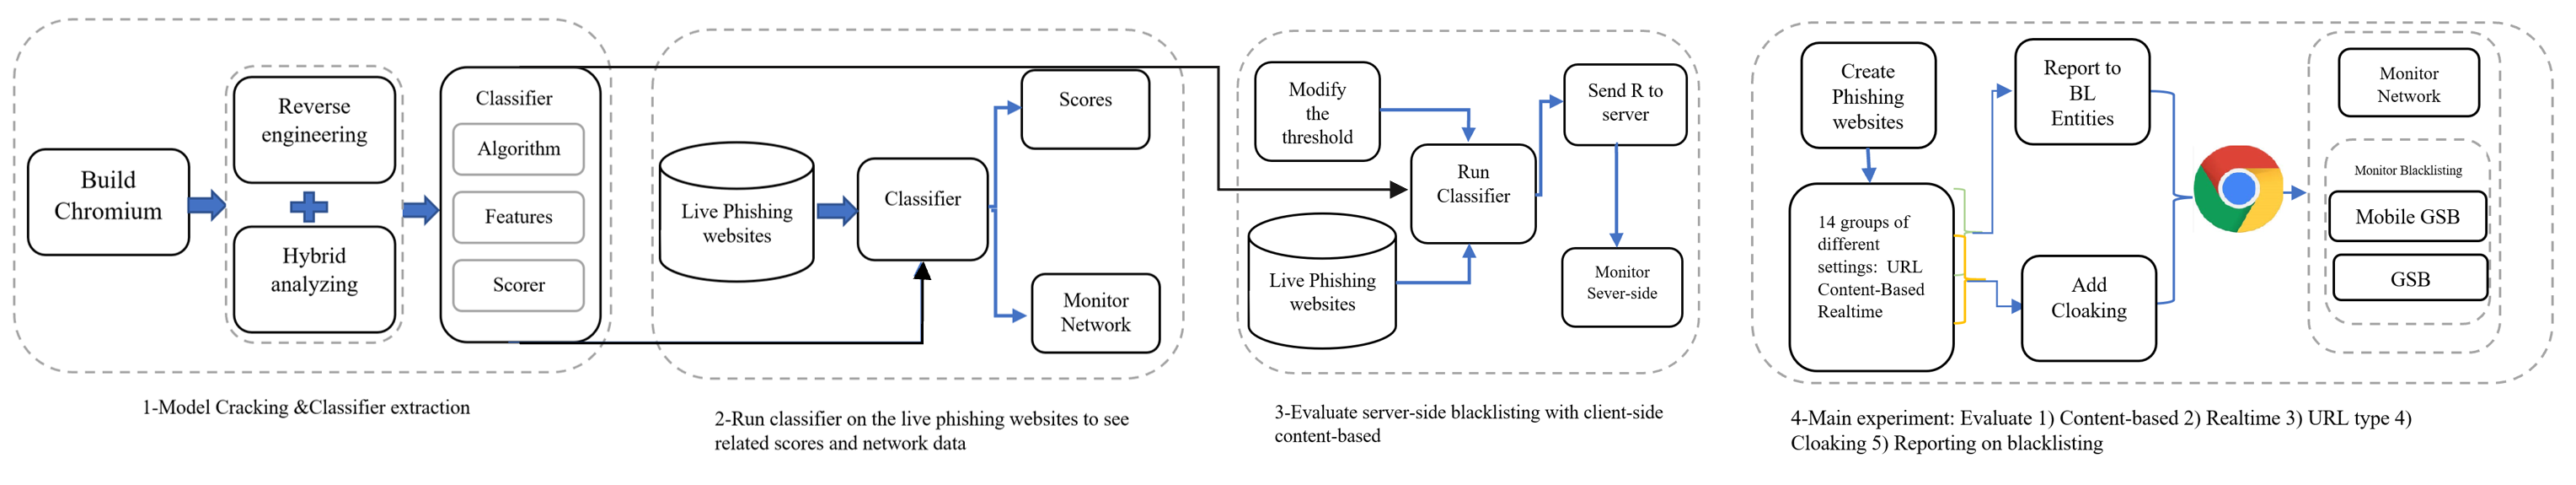
\includegraphics[width=\textwidth,height=5cm]{Overallscheme1.png}
%   \caption{ Client-side Content-based Anti-phishing Analyzing}
% \end{figure*}
% \lipsum[3-10]


\begin{table*}
\centering
\scalebox{0.9}{
\begin{tabular}{lll} 
\hline
\toprule
\textbf{Feature}                                    & \textbf{Brower features}                     & \textbf{Description of the features}                                                                                                                                                                             \\ 
\hline
\multirow{8}{*}{History features}            & kUrlHistoryVisitCount               & Number of visits to that URL stored in the browser history                                                                                                                                              \\
                                             & kUrlHistoryTypedCount               & Number of times the URL was typed in the Omnibox                                                                                                                                                        \\
                                             & kUrlHistoryLinkCount                & Number of times the URL was reached by clicking a link                                                                                                                                                  \\
                                             & kUrlHistoryVisitCountMoreThan24hAgo & Number of times URL was visited more than 24h ago                                                                                                                                                       \\
                                             & kHttpHostVisitCount                 & \multirow{2}{*}{\begin{tabular}[c]{@{}l@{}}Number of user-visible visits to all URLs on the same host/port as\\~the URL for HTTP and HTTPS \end{tabular}}                                               \\
                                             & kHttpsHostVisitCount                &                                                                                                                                                                                                         \\
                                             & kFirstHttpHostVisitMoreThan24hAgo   & \multirow{2}{*}{\begin{tabular}[c]{@{}l@{}}Boolean feature which is true if the host was visited for the first~\\time more than 24h ago (only considers user-visible visits like above) \end{tabular}}  \\
                                             & kFirstHttpsHostVisitMoreThan24hAgo  &                                                                                                                                                                                                         \\ 
\hline
\multirow{13}{*}{Browse features           } & kHostPrefix                         & \begin{tabular}[c]{@{}l@{}}prefixes appended to~features that tell for which page type\\~the feature pertains\end{tabular}                                                                              \\
                                             & kReferrer                           & Referrer                                                                                                                                                                                                \\
                                             & kHasSSLReferrer                     & True if the referrer was stripped because it is an SSL referrer                                                                                                                                         \\
                                             & kPageTransitionType                 & Stores the page transition                                                                                                                                                                              \\
                                             & kIsFirstNavigation                  & True if this navigation is the first for this tab                                                                                                                                                       \\
                                             & kRedirectUrlMismatch                & \begin{tabular}[c]{@{}l@{}}Feature that is set if the URL from the navigation entry doesn't match\\~the~URL at the end of the redirect chain\end{tabular}                                               \\
                                             & kRedirect                           & The redirect chain that leads to the named page                                                                                                                                                         \\
                                             & kSecureRedirectValue                & \begin{tabular}[c]{@{}l@{}}If a redirect is SSL, we will use this value instead of the actual redirect\\~so we don't leak any SSL sites\end{tabular}                                                    \\
                                             & kHttpStatusCode                     & The HTTP status code for the main document                                                                                                                                                              \\ 
\cline{2-3}
                                             & kSafeBrowsingMaliciousUrl           & \multirow{4}{*}{Fields from the UnsafeResource if there is~any}                                                                                                                                         \\
                                             & kSafeBrowsingOriginalUrl            &                                                                                                                                                                                                         \\
                                             & kSafeBrowsingIsSubresource          &                                                                                                                                                                                                         \\
                                             & kSafeBrowsingThreatType             &                                                                                                                                                                                                         \\
\hline
\end{tabular}}
\caption{Browser features}
\label{tab:Browser features}
\end{table*}

\subsection{Cracking Client-Side model}

% Since the public knowledge about the structure of google safe browsing client-side anti-phishing is rare, we decided to study this ecosystem by directly investigating Chromium, a development version of the chrome browser.
% To study the structure of google safe browsing client-side anti-phishing, we investigated the Chromium. Chromium is a development version of the Chrome browser

We interpreted the network traffic data as well as reverse-engineered the classifier using dynamic and static analysis on chromium source code to analyze the client-side content-based anti-phishing.
To study the client-side anti-phishing mechanism, we extract the features that this classifier uses for detecting phishing websites. There are two types of features in the client-side anti-phishing mechanism. The first group of features is used by the client-side classifier to compute the website's phishy-ness score. To study the structure of google safe browsing client-side anti-phishing which was neglected in previous studies, we investigated Chromium. Chromium is a development version of the Chrome browser. 
% The second part of the classifier is the algorithm. 

% To get a clear picture of the google safe browsing client-side anti-phishing, we built the Chromium source code as well as debugging, performed static and dynamic analysis, and interpreted the network data.

% After building the chromium source code, we perform static and dynamic analyzing, logging and debugging, and network data interpretation we make a clear picture of google safe browsing client-side anti-phishing mechanism.
We analyzed the classifier in real-time after opening 100 live phishing websites from Phishtank to extract which features are responsible for detecting the malicious websites. Moreover, the values and weights of those features were estimated.
% Running this analysis for 100 live phishing websites from Phishtank, we partially cracked the model by finding the extracted features and related value and weight. 
%%% outline{ In this subsection, we explain how and why we try to crack the classifier's model:

% Partially crack the new model with build chromium source code +static analyzing+ debugging + dynamic analyzing.

% Extract classifier algorithm 

% Scorer formula 

% Features

% GSB databases }

\begin{table}
\centering
\scalebox{0.83}{
\begin{tabular}{lcc} 
\hline
\toprule
              & {Old Model}                                                                         & {New model}                                                                                         \\ 
\hline
\small{Model version} & \small{5}                                                                                  & \small{5X}                                                                                                \\
\small{Rule Numbers}  & \small{2130}                                                                               & \small{3100}                                                                                              \\
\small{Threshold}     & \begin{tabular}[c]{@{}c@{}}\small{Static}\\\small{Threshold}\textbf{\textit\small{{ = 0.5}}}\\~\end{tabular} & \begin{tabular}[c]{@{}c@{}}\small{Dynamic}\\\small{Current Threshold= 0.8999976} \\~\end{tabular}             \\
\small{Features}      & \small{URL-DOM-Term}                                                                       & \small{URL-DOM-Term-Visual~}                                                                              \\
\small{Phishy-ness~}  & \small{score} \textgreater{}= \small{Threshold}                                                                  & \begin{tabular}[c]{@{}c@{}}\small{score} \textgreater{}= \small{ Threshold} \small{or~}\\\small{Visual Target Match}\end{tabular}  \\
\bottomrule
\end{tabular}}
\caption{Difference between the new model and the old model}
\label{ModelDifference}
\end{table}


\subsubsection{Features} 

Client-side content-based anti-phishing uses two type of features:
\begin{enumerate}
\item Model and page (classifier-related) features Chrome client-side content-based anti-phishing classifier uses three type of features in computing the final score.
    \begin{enumerate}
    \item URL features: This type of features make reference to some attributes of the URL.
    \item DOM Features: Client-side classifier uses the Document Object Model (DOM) elements of the page as some features for computing the phishy-ness score. In table \ref{tab:Dom features}, we show all 13 kinds of DOM features employed by chrome.
    \item Term Features: Client-side classifier uses the terms in the page as a kind of feature. This feature refers to a single word or a combination of multiple words (maximum five words).
\end{enumerate}
\item Browser features: After running the classifier on the web page features by the renderer, if the final score is higher than the threshold browser extracts the browser features. Browser features refer to 21 features that are shown in table \ref{tab:browser features}. Browser appends these features to the classifier results and send the phishing request to the server. These features include history, navigation, redirection and safe browsing related features.
    
\end{enumerate}

% \usepackage{multirow}




\begin{table*}
\centering
\scalebox{0.95}{
\begin{tabular}{lll} 
\toprule
 \textbf{DOM feature type}                                                           & \textbf{Model DOM features}  & \textbf{Page DOM features}                                                                                                                              \\ 
\hline
\multirow{7}{*}{\begin{tabular}[c]{@{}l@{}} DOM HTML\\form features \end{tabular}}   & PageHasForms                 & Page has any form element                                                                                                                               \\
                                                                                     & PageActionOtherDomainFreq    & \begin{tabular}[c]{@{}l@{}}The fraction of form elements whose “action" attribute\\ point URL on a different domain \end{tabular}      \\
                                                                                     & PageActionURL                & \begin{tabular}[c]{@{}l@{}}The token feature containing each URL\\that an “action" attribute points to \end{tabular}  \\
                                                                                     & PageHasTextInputs            & The page has any input type=“text" element                                                                                                              \\
                                                                                     & PageHasPswdInputs            & The page has any input type=“password" element                                                                                                          \\
                                                                                     & PageHasRadioInputs           & The page has any input type=“radio" element                                                                                                             \\
                                                                                     & PageHasCheckInputs           & The page has any input type=“checkbox" element                                                                                                          \\ 
\hline
\multirow{3}{*}{\begin{tabular}[c]{@{}l@{}} DOM HTML\\link features \end{tabular}}   & PageExternalLinksFreq        & The fraction of links on the page that point\textasciitilde{} to other domains                                                                          \\
                                                                                     & PageLinkDomain               & The token feature containing each external domain that is linked to                                                                                     \\
                                                                                     & PageSecureLinksFreq          & The fraction of links on the pageدthat use HTTPS                                                                                                        \\ 
\hline
\multirow{2}{*}{\begin{tabular}[c]{@{}l@{}} DOM HTML\\script features \end{tabular}} & PageNumScriptTagsGTOne       & The number of script elements on the page is greater than 1?                                                                                            \\
                                                                                     & PageNumScriptTagsGTSix       & The number of script elements on the page is greater than 6?                                                                                            \\ 
\hline
\begin{tabular}[c]{@{}l@{}}Other DOM\\HTML features \end{tabular}                    & PageImgOtherDomainFreq       & \begin{tabular}[c]{@{}l@{}}The fraction of images whose source attribute\\\textasciitilde{}points to an external domain \end{tabular}                   \\
\bottomrule
\end{tabular}}
\caption{DOM features}
\label{tab:Dom features}
\end{table*}
%%%%%%%%%%%%%






\subsubsection{Algorithm}

Combining static and dynamic analysis, we extract the classification algorithm. The client-side content-based anti-phishing has two phases:

\begin{enumerate}
    \item Pre-classification: Client-side anti-phishing classification starts with some checks in the pre-classification phase. As shown in figure \ref{fig:Pre-classification}, it classifies only [X]HTML documents and HTTP/S pages. It does not classify any tab in incognito or any  URL in whitelisted by enterprise policies, or any URL is in the local Client-side detection whitelist database, and it does not classify for the private IPs.
    
    \item Main classification: In the first step, the client-side content-based anti-phishing runs a pre-classification on the webpage; after passing these conditions, the main classification starts. Client-side suppose Safe Browsing client-side phishing detector distinguishes that the webpage is similar to phishing pages according to the client-side detector machine learning model's results. In that case, it will send a request to the Safe Browsing server to ask the server to make a final decision about the page. If Safe browsing detects the page as a phishing page, the browser shows a warning page.

\begin{figure}[!h]
\centering
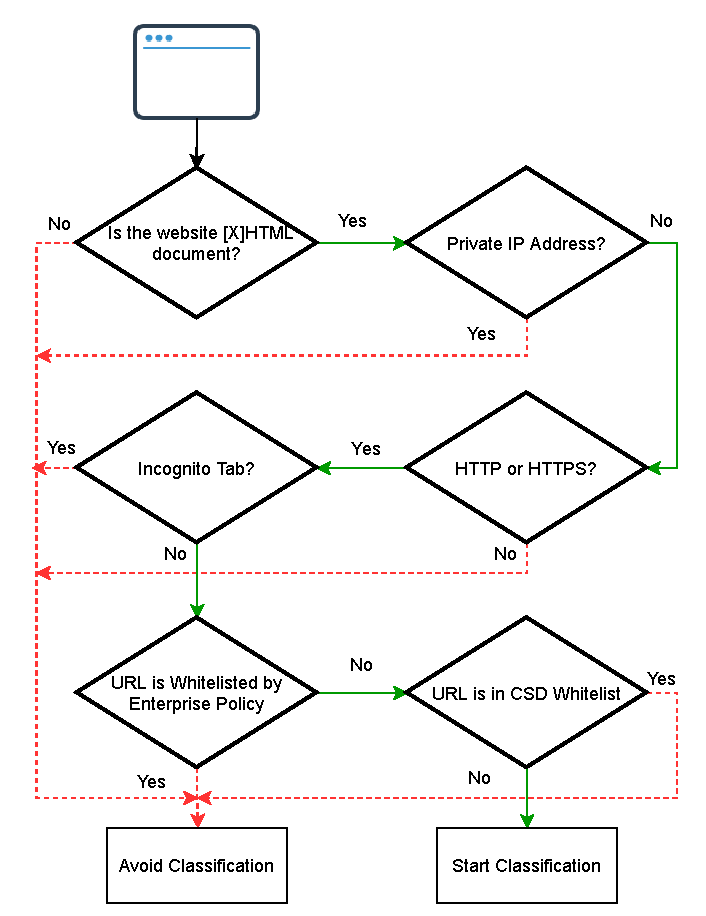
\includegraphics[height=4.5in, width=3in]{preclassificationdiagram-3.pdf}
\caption{Pre-Classification algorithm}
\label{fig:Pre-classification}
\end{figure} 
We found out that the classifier's algorithm has changed compared to the findings of the previous work during our analysis.
Client-side classifier extracts the third type of features, which is called visual features.  It downloads the client-side model's visual target map and compares the visual features with the visual targets. If the features match, the client-side content-based anti-phishing supposes the site as a malicious website and sends the request to the server-side to analyze the site.
\end{enumerate}

\begin{figure}[h!]
\centering
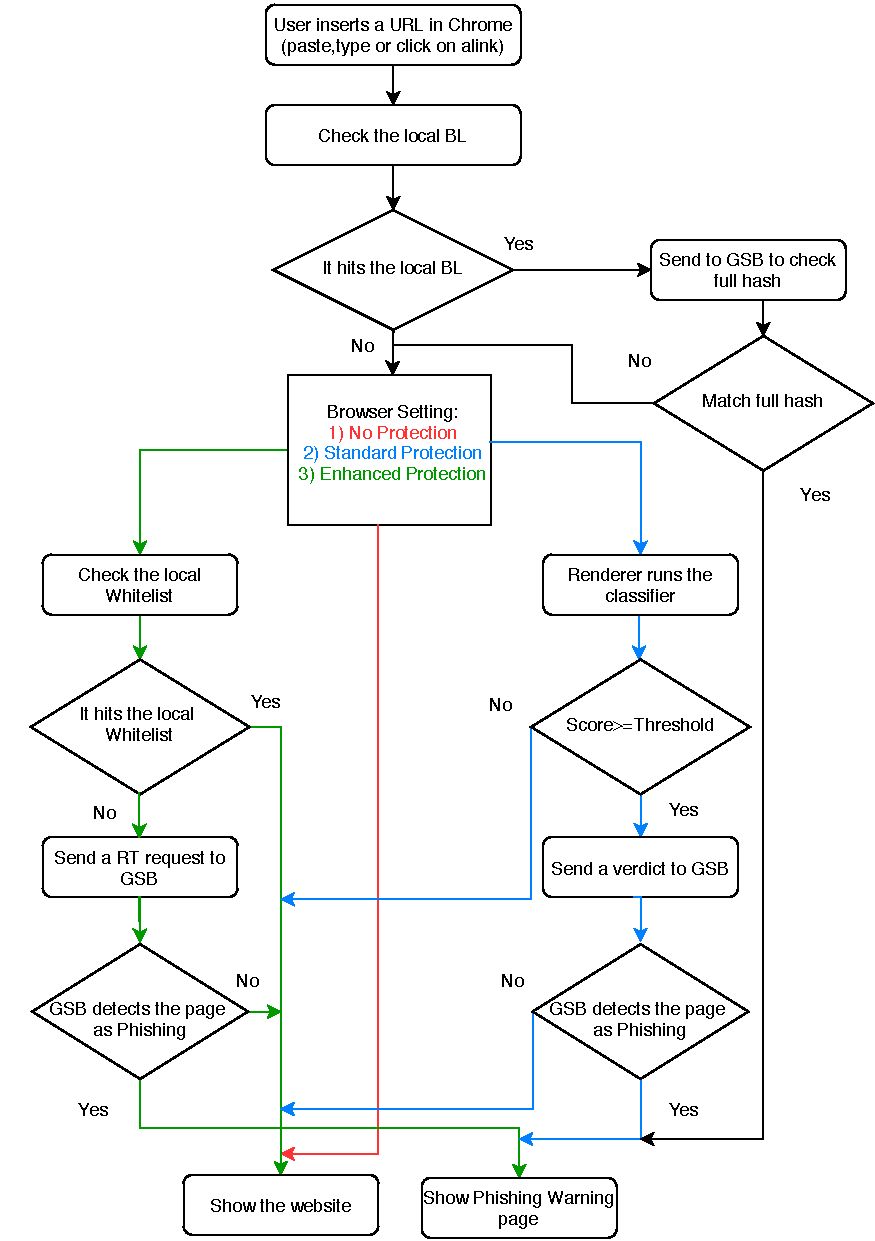
\includegraphics[height=5.0in, width=2.9in]{chrome-ecosystem.pdf}
\caption{Chrome Client-side anti-phishing ecosystem}
\label{fig:Chrome client side anti-phishing flowchart}
\end{figure} 

In the new version of client-side content-based anti-phishing, the classifier uses visual features. As shown in figure \ref{fig:visual features} The classifier detects the related website as a malicious website in two conditions:
\begin{enumerate}
    \item If the score of the website is above the threshold
    \item If the visual features match the visual target
\end{enumerate}

 \begin{figure}[h!]
\centering
\scalebox{0.9}{
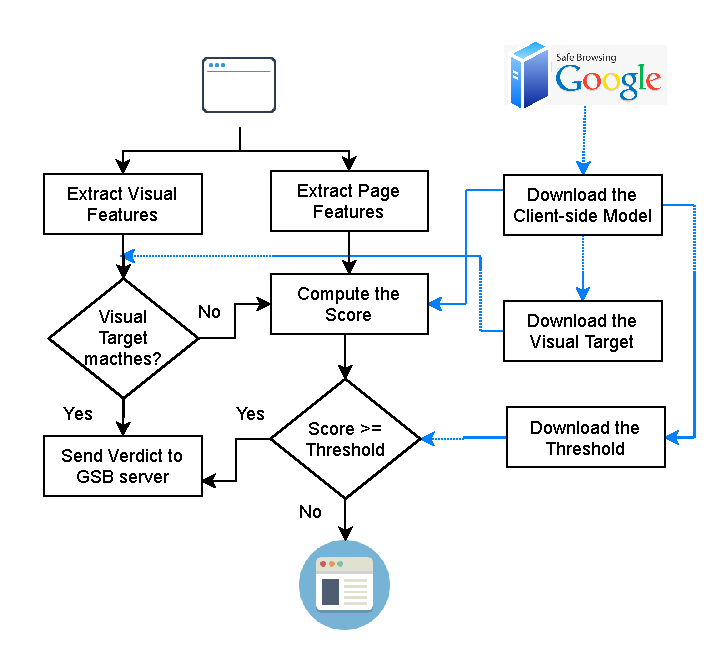
\includegraphics[height=3.7in, width=3.5in]{Visual target (1).pdf}}
\caption{Visual features' role in client-side content-based anti-phishing}
\label{fig:visual features}
\end{figure} 

\subsection{Evaluating client-side Classifier Results}
To measure the client-side content-based anti-phishing, we extracted the classifier, analyzed it with a bunch of phishing websites, and recorded the classifier's final decision besides the scorer's results.
We used 100 phishing websites from Phishtank database for this purpose.
We ensured that similar phishing websites were not duplicated across these URLs.
% We have done this for the first 10 phishing websites pf the phishtank in 10 weeks to minimize the risk of doing classification for similar phishing websites. 
% On September 2020 when we realized the client-side anti-phishing model have changed, we repeated the experiment for other 100 phishing website from phishtank in a similar way. 

% We consider two factors to compare the results of the classifier for old and new phishing websites:
% \begin{enumerate}
%     \item Improvement of the model(as a positive factor on classifier results)
%     \item The increasing of the phishers knowledge (as a negative factor on classifier results)
% \end{enumerate}

\subsection{Evaluating Server-Side Classifier Results}
%we show the performance of client-side content based anti-phishing system
To evaluate the server-side classifier, we send many live phishing websites to the server-side classifier and analyzed the server's response to the client. For this purpose, we Modified the phishing threshold to zero to make the browser send the request to the server-side. At technical level,  we modified the threshold in the source code and recompiled the Chromium binary file, visited 100 phishing websites, and captured the server responses using a proxy. For making more promising decision, we recorded the client-side classifier scores of all the phishing websites.

% We feed the server-side classifier with client-side requests and monitor the server response using Proxy and browser behavior.
\subsection{Password Protection Anti-phishing}
We analyze the phishing websites' HTML files that we fed to the client-side password-protection anti-phishing during our experiment. After performing hybrid analysis on chromium source code and monitoring the network data with BurpSuit proxy beside this analysis, we found out this mechanism has a significant weakness. If the DOM element name in the page is not ``password", the password protection does not carry out a password-exposure check nor phishing classification for that page.  
\subsection{Real-time Anti-phishing evaluation}

In September 2019, chrome version 79 came with a new defense layer against phishing websites. Google to cover the blacklist refreshing windows and preventing the attackers from exploiting that approximately 30 minutes refreshing time to perform their new attacks, or continue their attacks by continuously changing their domains, presented the real-time anti-phishing method.
Having chrome version 79 or newer, when users visit a website, Chrome checks it against the whitelist database on the user's system. 
In Chrome version 79 or newer, Chrome sends the URL to safe browsing unless it is on a whitelist. The whitelist is stored locally and includes thousands of popular websites that are known to be safe. If the visited website's URL does not match with the local whitelist database, the browser sends the URL to the google safe browsing server to check if the user is visiting a malicious website.~\cite{gsbapi,googlechromeprivacywhitepaper}. 
In this study, we consider real-time in the browser settings in the blacklisting experiment to evaluate its effect on blacklisting performance.
% coverage and speed. 
We also evaluate the empirical experiment on 50 phishing websites and monitor the chrome behavior, the real-time request that the browser sends, and the server results.

\subsection{Measuring Blacklist performance}
%{Speed and Coverage}
%we show the content-based anti-phishing effects on blacklisting coverage and speed
It is the central part of the experiment:
For the 14 batches domains, we use different combinations of the browser-side anti-phishing mechanisms, cloaking, and reporting to evaluate the effects of client-side anti-phishing methods, including client-side content-based and real-time anti-phishing, cloaking as the most popular evasion method and reporting on the blacklisting performance.
% speed and coverage.

This analysis seeks to figure out how effective client-side content-based anti-phishing is in blacklisting and protecting the user from phishing websites. Also, How effective client-side content-based anti-phishing is in dealing with cloaking as an evasion technique.

\subsection{Privacy Issues in Client-Side Anti-Phishing }

In the phishing context, attackers need to gain user's sensitive and private information. However, anti-phishing techniques like Google Safe Browsing client-side anti-phishing claims that it protects user's sensitive information~\cite{googlechromeprivacywhitepaper}, but in reality, Chrome browser does not give the true sense of trust to the users and does not entirely guarantee the privacy of the user's activities.
We analyze client-side anti-phishing behavior in user privacy in two different scenarios:
\begin{enumerate}
    \item User privacy in phishing detection for every un-seen website
    \item User privacy in password protection mechanism
\end{enumerate}

\subsubsection{Privacy issue in client-side anti-phishing detection} 

When the client-side anti-phishing classifier computes the page's phishy-ness score, the pages with a score above the threshold browser send a request to the server to check the page and respond with the final decision about the page's phishy-ness score. 
Our experiments show that this request includes the page URL, referring URL, as well as technical parameters about the classifier and classification results such as:
1) Feature Map
2) Client Score
3) Model version
4) Browser features
5) URL
6) The client-side classifier result
7) Vision match result
8) Feature map size
9) Non-model feature map
10) Non-model feature map size
11) Referrer URL
12) Shingle hashes size
13) Shingle hashes
14) Model file name
This request includes the visited URL.
% Figure~\ref{fig:Phishing Request to the server} shows a screenshot of proxy showing the sent phishing request to the Google Safe Browsing. 
However, google chrome informs the user about the information it sends to the server under the related setting.

% \begin{figure}
% \centering
% \includegraphics[width=3in,height=2.5in]{Reporttoserver.png}
% \caption{Phishing Request to the server}
% \label{fig:Phishing Request to the server}
% \end{figure} 

\subsubsection{Privacy issue in client-side password protection }
Password protection is not enabled on the chrome browser setting. Having chosen this protection by the user, if a user clicks on the password box, client-side password protection starts running phishing classification on the page regardless of previous pre-classification results~\cite{mardini_2019}. 
Our experiments show that when users insert a password, the browser sends the visited URL and URLs of all the websites with the same saved password to google safe browsing.   
However, the client-side password protection mechanism eliminates user's information includes user names and passwords. It exposes users' current and previous activities related to the password to the google safe browsing server. The revealed privacy issue is not disclosed to the user in the chrome browser settings where the user should enable this mechanism.
%%%% Outline{ This section focuses on:
% Leveraging privacy issues on client-side content-based anti-phishing
% What user data browser sends to the server in the client-side anti-phishing mechanism } outline 

\section{Implementation of Experiments}
In the preliminary experiment, we extracted a total of 200 newest and not blacklisted phishing websites 10 per week from the Phishtank database, 100 for the client-side analysis, and 100 for server-side classifier evaluation. 
For the blacklisting experiment, we adjusted a previously-conducted test framework(Phishfarm \cite{oest2019phishfarm}) to establish our needed phishing websites.
To empirically measure blacklisting coverage and speed
and evaluate browser-based defenses such as blacklisting, content-based, and real-time anti-phishing, the testbed facilitates the configuration, development, API-based reporting, and monitoring of the nondangerous phishing websites.  We enhanced the testbed to support automation of monitoring the network, cloaking, and API-based reporting to accurately imitate current phishing trends and ecosystem defenses.

\subsection{Overview}
%%Outline{ We describe how we implement the experiment with technical details:
% First: How we get the phishing websites:
% we have two types of phishing websites:
% Database of phishing websites from "Phishtank."%}Outline
%We provide an overview of the experiment in figure 3
Our experiment is divided into the following steps: 
First, we designed 14 groups to entirely cover the features we want to evaluate their effects on the blacklisting process. Second deployed phishing websites using Phishfarm test-bed, 
To reduce the chances of being blacklisted due to the domain's low reputation, we used the domains a month later.
We deploy the network monitor tools in the VMs, then activated the websites. Over the next seven days, we monitor the blacklist status, and we log the crawler traffic.
At the last step of the blacklist experiment, we deactivated the websites and analyzed the log file.

\subsection{Client-side and server-side Classifier evaluation}
% In this section, we show:

% How we extract the classifier from the chromium and build the chrome file to run the classifier

% How to modify the threshold
As an open-source project, we are able to compile chromium source code to achieve a debug version, including symbols of functions, variables, algorithms, databases, and structures. In this paper, we use visual studio as the debug tool. We explore the Safe Browsing folder in the source code to locate client-side anti-phishing files, data structures, and debugging points. 
The multi-layer architecture prevents to crack all anti-phishing components by static analysis. Extracting model and page features, setting threshold, computing the score, and checking the visual target matches are accrued in the renderer process. On the other hand, pre-classification checks, loading machine learning model, password protection process, browser feature extraction, Sending the classification request to the renderer process, receiving the results, and finally sending phishing requests to the server are implemented in the browser process.
We omitted some extracted sensitive details of chrome client-side anti-phishing intentionally to prevent them from being used by malicious users. 

\subsection{Blacklist Monitoring}

To empirically monitor blacklisting speed and coverage
of phishing websites, We used the adapted previous-presented test-framework( Phishfarm) \cite{oest2019phishfarm} on a total of 8 virtual machines(VMs). We modified chrome browser anti-phishing settings on each VM to perform a blacklisting monitor with different anti-phishing techniques.
% In this section, we describe:

% How we monitor the blacklisting process: We use the Phishfarm framework.

% we monitor :

% desktop and mobile blacklists

\subsection{Network Monitoring}

To study privacy-related issues in the client-side content-based anti-phishing, we implement a proxy to monitor the network during the blacklist experiment. We used BurpSuit for the windows platform in the preliminary experiment and MITMproxy during the main experiment on the Ubuntu systems. To verify that no traffic bypassed the proxy in the chrome browser, we also employed Wireshark to capture network data.
 
\begin{table*}[t]
\centering
\scalebox{0.95}{
\begin{tabular}{ccccccccc} 
\hline
\toprule
                     & \multicolumn{5}{c}{Experiment Settings}                                                                                                                                                            & \multirow{4}{*}{\begin{tabular}[c]{@{}c@{}}Total Number of\\Websites per group\end{tabular}} & \multirow{4}{*}{\begin{tabular}[c]{@{}c@{}}Number of\\Blacklisted\\websites:\\ChromeBlacklist\end{tabular}} & \multirow{4}{*}{\begin{tabular}[c]{@{}c@{}}Number of\\Blacklisted\\websites:\\mGSBBlacklist\end{tabular}}  \\ 
\cline{1-6}
                     & \multirow{3}{*}{URL~} & \multirow{3}{*}{CB} & \multirow{3}{*}{RT} & \multirow{3}{*}{Report~} & \multirow{3}{*}{Evasion Technique}                                                                  &                                                                                              &                                                                                                             &                                                                                                           \\
\multicolumn{1}{l}{} &                       &                     &                     &                          &                                                                                                     &                                                                                              &                                                                                                             &                                                                                                           \\
\multicolumn{1}{l}{} &                       &                     &                     &                          &                                                                                                     &                                                                                              &                                                                                                             &                                                                                                           \\ 
\hline
\small{1}  & \small{Rand} & \cmark & \xmark  & \xmark      & \small{Cloaking}                                                                                            & \small{35}                                                                                           & {\cellcolor[rgb]{1,0.49,0.49}}\small{0}                                                                             & {\cellcolor[rgb]{1,0.49,0.49}}\small{0}                                                                           \\
\small{2}  & \small{Rand} & \cmark &\xmark  & \xmark      & \small{No Cloaking}                                                                                            & \small{35}                                                                                           & {\cellcolor[rgb]{1,0.49,0.49}}\small{0}                                                                             & {\cellcolor[rgb]{1,0.49,0.49}}\small{0}                                                                           \\
\small{3}  & \small{Susp} &  \cmark & \xmark  & \xmark      & \small{No Cloaking}~                                                                                        & \small{35}                                                                                          & {\cellcolor[rgb]{1,0.49,0.49}}\small{0}                                                                             & {\cellcolor[rgb]{1,0.49,0.49}}\small{0}                                                                           \\
\small{4}  & \small{Rand} &  \cmark &  \cmark & \xmark      & \small{No Cloaking}                                                                                        &  \small{35}                                                                                           & {\cellcolor[rgb]{1,0.49,0.49}}\small{0}                                                                             & {\cellcolor[rgb]{1,0.49,0.49}}\small{0}                                                                           \\
\small{5}  & \small{Susp} & \cmark & \cmark & \xmark     & \small{Cloaking}                                                                                             & \small{35}                                                                                           & {\cellcolor[rgb]{1,0.49,0.49}}\small{1}                                                                             & {\cellcolor[rgb]{1,0.49,0.49}}\small{0}                                                                           \\
\small{6}  & \small{Rand} & \cmark & \cmark & \cmark     & \small{No Cloaking}                                                                                         & \small{35}                                                                                           & {\cellcolor[rgb]{0.592,0.867,0.592}}\small{33}                                                                      & {\cellcolor[rgb]{0.592,0.867,0.592}}\small{35}                                                                    \\
\small{7}  & \small{Susp} &\xmark  &  \cmark &  \cmark     & \begin{tabular}[c]{@{}c@{}}\small{No Cloaking} \\\small{+ Not visible} \\\small{to the Client-side Classifier}\end{tabular} & \small{35}                                                                                           & {\cellcolor[rgb]{0.592,0.867,0.592}}\small{34}                                                                      & {\cellcolor[rgb]{1,0.49,0.49}}\small{0}                                                                           \\
\small{8}  & \small{Susp} & \cmark & \cmark & \cmark     & \small{No Cloaking}                                                                                         & \small{35}                                                                                           & {\cellcolor[rgb]{0.592,0.867,0.592}}\small{34}                                                                      & {\cellcolor[rgb]{0.592,0.867,0.592}}\small{31}                                                                    \\
\small{9}  & \small{Susp} & \cmark & \cmark & \cmark     & \small{No Cloaking}                                                                                         & \small{35}                                                                                           & {\cellcolor[rgb]{0.592,0.867,0.592}}\small{34}                                                                      & {\cellcolor[rgb]{0.592,0.867,0.592}}\small{33}                                                                    \\
\small{10} & \small{Rand} & \cmark & \xmark  & \cmark     & \small{Cloaking}                                                                                             & \small{35}                                                                                           & {\cellcolor[rgb]{0.592,0.867,0.592}}\small{35}                                                                      & {\cellcolor[rgb]{1,0.49,0.49}}\small{0}                                                                           \\
\small{11} & \small{Susp} & \cmark & \xmark  & \cmark     & \small{Cloaking}                                                                                             & \small{35}                                                                                           & {\cellcolor[rgb]{0.592,0.867,0.592}}\small{35}                                                                      & {\cellcolor[rgb]{1,0.49,0.49}}\small{2}                                                                           \\
\small{12} & \small{Rand} & \cmark & \xmark  & \cmark     & \small{No Cloaking}                                                                                         & \small{35}                                                                                           & {\cellcolor[rgb]{0.592,0.867,0.592}}\small{35}                                                                      & {\cellcolor[rgb]{0.592,0.867,0.592}}\small{33}                                                                    \\
\small{13} & \small{Rand} & \xmark  & \cmark & \cmark     & \small{Cloaking}                                                                                             & \small{35}                                                                                           & {\cellcolor[rgb]{0.592,0.867,0.592}}\small{35}                                                                      & {\cellcolor[rgb]{1,0.49,0.49}}\small{0}                                                                           \\
\small{14} & \small{Rand} & \xmark  & \cmark & \cmark     & \begin{tabular}[c]{@{}c@{}}\small{No Cloaking} \\+ \small{Not visible}\\\small{~to the Client-side Classifier}\end{tabular} & \small{35}                                                                                           & {\cellcolor[rgb]{0.592,0.867,0.592}}\small{35}                                                                     & {\cellcolor[rgb]{0.592,0.867,0.592}}\small{31}                                                                   \\
\bottomrule
\end{tabular}}
\caption{Blacklisting coverage results}
\label{fig:coverage results}
\end{table*}


\section{Experimental Results}

Several experiments on various aspects of client-side anti-phishing indicate client-side classifier's inefficacious proficiency, insufficient features used in classifiers, ineffective server-side results, and the efficacy of content-based and real-time anti-phishing in desktop and mobile blacklisting.

\subsection{ Client-side classifier Detection Accuracy }

%%% Outline{ In this section, we show:

% False Negative results of the classifier

% the results of a scorer for 100 phishing websites( we use a figure to show the distribution of the scores)

% The percent of phishing websites with a score higher than the threshold ( we use a figure to show the classification results of the classifier) %%% } Outline 
The classifier's result for 100 phishing websites shows that chrome client-side content-based anti-phishing could not detect 85\%  of phishing websites. This experiment signifies that the classifier has remarkable False Negative results. 
\begin{table}[]
\scalebox{0.8}{
\begin{tabular}{|c|c|c|}
\hline
\begin{tabular}[c]{@{}c@{}}Number of \\ Phishing websites\end{tabular} &
  \begin{tabular}[c]{@{}c@{}}Client-side classifier\\  result\end{tabular} &
  \begin{tabular}[c]{@{}c@{}}Sever-Side classifier\\  result\end{tabular} \\ \hline
100 &
  15\% &
  7\% \\ \hline
\end{tabular}%
}
\caption{Client-side and server-side detection ratio}
\label{tab: Client -side and server-side}
\end{table}

After our first experiment and the continuous dynamic analysis of chromium, we realized that the google safe browsing client-side phishing detection model has changed. 
Table \ref{ModelDifference} shows the difference between the new model and the old model. One of the most important changes in the new model is tuning the threshold.
Client-side anti-phishing detection does not use a static threshold ( which was 0.5) to identify the phishing sites. In the new model, google safe browsing tunes the threshold and send a dynamic threshold to the client. 
We confirm that classifier sets the threshold in function~\textit{threshold-probability()} which is a method of the \textit{Scorer} class defined in the file \textit{scorer.cc}. 
% % csd.pb.h protocol buffer 
% \textbf{\emph{accident}}
% \textit{Scorer.cc } file sets the threshold by calling the   \textit{model.threshold_probability()} function. 
Figure \ref{fig:two model} shows the results of the classifier with the old model and new model results. Although the scorer results are mainly changed, the dynamic threshold (During our experiment in late September, the model threshold was 0.88) became larger than the old static threshold(0.5). Therefore, the number of sites with the phishy score ( scores higher than the threshold) is noticeably low.
As shown in figure \ref{fig:two model} accuracy in the new model is improves by 35\%. 

 \begin{figure}
\centering
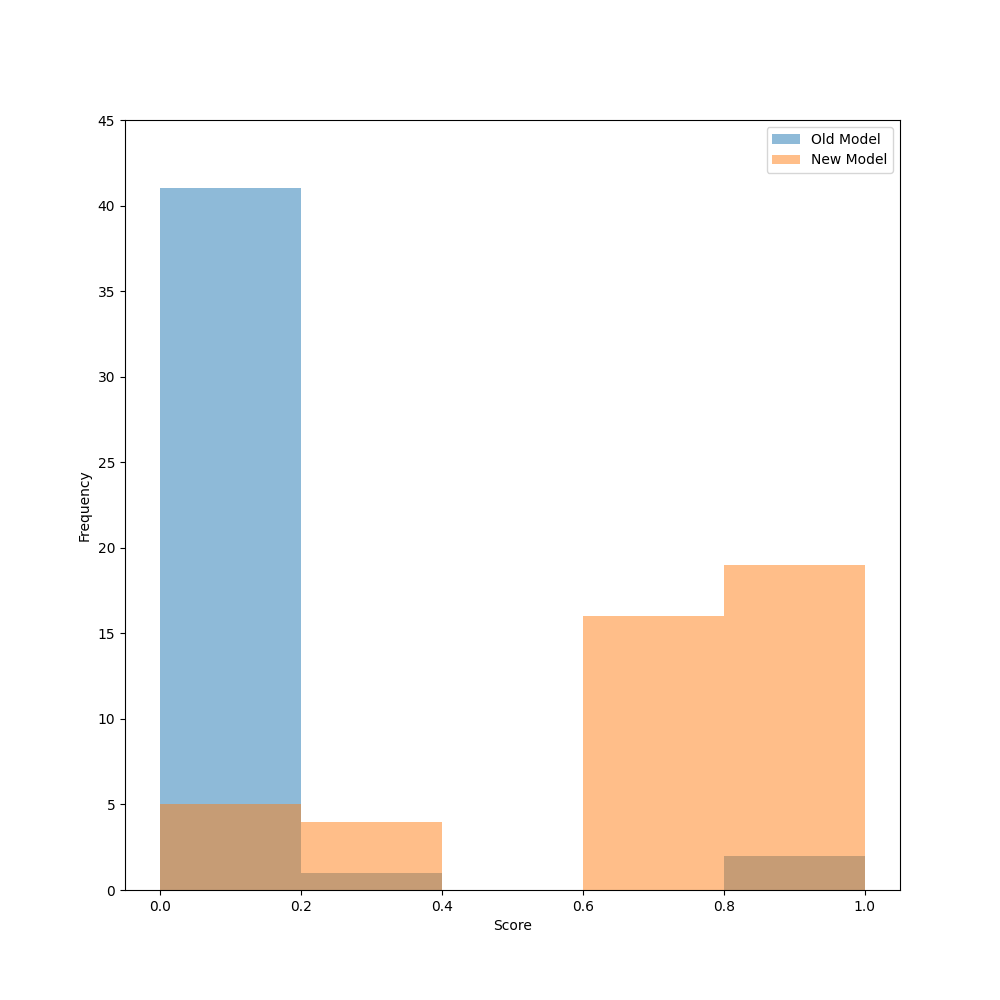
\includegraphics[height=3in, width=3in]{image (1).png}
\caption{The scorer results in two model }
\label{fig:two model}
\end{figure} 

\subsection{Overall Client-side Content-based Anti-phishing Performance}

%%% outline{ This subsection includes our main results:

% The figure of blacklisting progress during the experiment for 14 batches%% outline}

as shown in \ref{fig:coverage results}, our experiment demonstrates:
\begin{enumerate}
    \item The websites in groups without reporting did not get blacklisted
    \item all groups of websites with content-based anti-phishing even with suspicious URLs did not get blacklisted
    \item The groups of websites with real-time anti-phishing even with suspicious URLs did not get blacklisted
\end{enumerate}
According to the network data files and the crawlers log file, the client-side classifier did not detect these websites as phishing websites. There are two main assumptions for this result:
a)Chrome did not run the classifier on these websites. It might be because avoiding classification when extracting the DOM features takes much time. According to the dynamic analysis of the chromium source code, we found out if extracting DOM elements takes a long time, the classifier runs RunFailure() function and skips the classification.
b)The classifier result score is less than the threshold. This assumption proves the weaknesses of the machine-learning model accuracy.  The client-side content-based anti-phishing accuracy experiment strengthens this assumption.

%%%%%%%%%%%Figure for the result table%%%%
% \begin{figure}
% \centering
% \scalebox{0.9}{
% \includegraphics[height=4in, width=3.5in]{Theresultofexperimentmobilechrome.png}}
% \caption{Blacklisting coverage results}
% \label{fig:coverage results}
% \end{figure} 
%%%{شاید البته مطمعن نیستم رو این قسمت 
%\subsection{Blacklist coverage}
%%%}
\subsubsection{Desktop Blacklists}

% In this section, we separately discuss the result of blacklisting for the desktop Blacklist providers.
Our study's primary goal is to identify the effect of client-side content-based anti-phishing on blacklisting the newborn phishing websites. After running the main experiment for seven days in mid-may 2020, we analyze the crawler log file and the framework results. Table \ref{fig:coverage results} presents the blacklist coverage for the desktop and mobile google safe browsing blacklists. The key finding in this experiment is the result of the first five groups. For 175 phishing websites, content-based anti-phishing does not affect the blacklisting coverage. For  35 suspicious URLs in group 5, using two client-side anti-phishing methods ( content-based and real-time), there is just one blacklisted phishing URL. The numbers of the blacklisted phishing URL confirm the inefficient performance of google safe browsing client-side anti-phishing methods. The first three groups use the default settings of the chrome browser. 
% The results for these three group shows the chrome 3 billion users' protection status against new phishing campaigns.

\subsubsection{Mobile Blacklists}
% In this section, we separately discuss the result of blacklisting for the mobile Blacklist providers.Mobile users
% To date, there have been no formal studies of the impact of cloaking on mobile google safe browsing blacklisting effectiveness.
The majority of Internet traffic users are mobile users~\cite{statcounterglobalstats}, and the earlier study has revealed that mobile web browsers are particularly vulnerable to phishing attacks~\cite{luo2017hindsight}.
% state the problem, what the new finding is, what the previous observation was, and then cite that
We point to one significant finding in our experiment; as shown in table~\ref{fig:coverage results}, none of the phishing sites that used cloaking became blacklist in theww  mobile chrome browsers while they blacklisted in the desktop chrome browsers. However, the inconsistency between desktop and mobile browsers blacklists of mobile chrome browser previously reported in 2018 by~\cite{oest2019phishfarm}, we showed that this shortcoming still exits.
For mobile chrome browsers with 61.35\%  of all mobile browsers, approximately 2.9 billion users worldwide, this finding is a crucial deficiency in the mobile chrome anti-phishing mechanism.
Although 90\%  of reported websites did blacklist on Desktop Google Safe Browsing, our experiment results showed that 95\%  of all the websites reported to the entities did not blacklist on Mobile Google Safe Browsing~\ref{fig:coverage results}.

\begin{figure*}[t]
  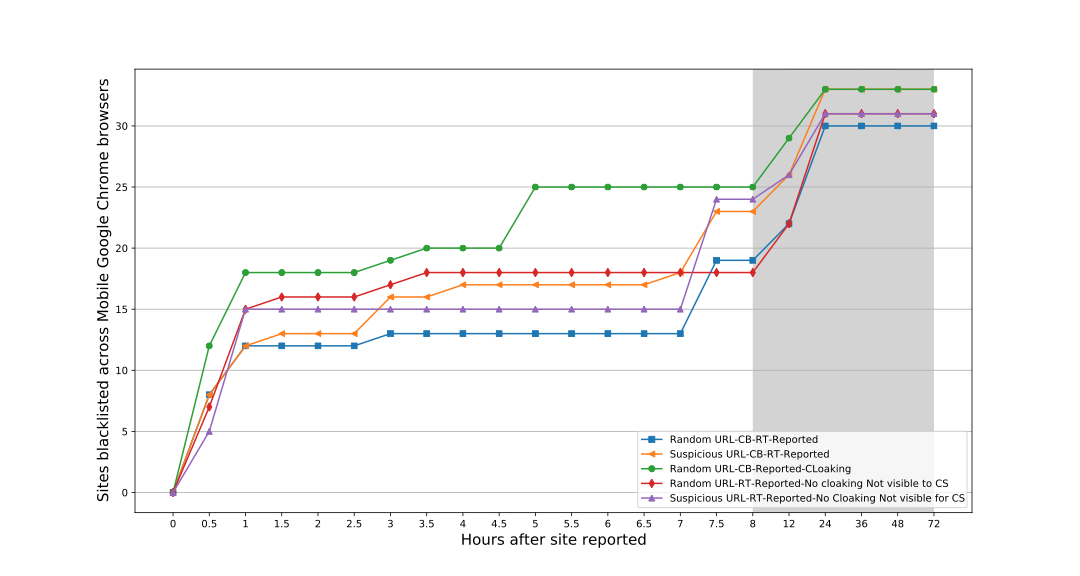
\includegraphics[width=\textwidth,height=9cm]{Mobile-Blacklists-Speed.png}
  \caption{Mobile Blacklisting Performance }
  \label{Blacklisting speed results}
\end{figure*}

%\subsubsection{Long-term Blacklist Consistency} 
\subsection{Blacklist speed}
The main goal of introducing client-side content-based anti-phishing is to cover the 30 minutes gap between updating the local blacklists. The result of our experiment shows that the number of blacklisted phishing websites in the first 30 minutes of the experiment for the not-reported one is zero.
Blacklisting speed for the reported phishing websites is presented in the figure \ref{Blacklisting speed results}. 

\subsection{Real-time anti-phishing evaluation}

Google claims the new real-time anti-phishing 30\%  improves the detection of the un-seen phishing websites. Our experiment results for the groups 5 and 6 ( as shown on the table \ref{fig:coverage results} for 70 phishing websites in these two groups, real-time anti-phishing does not affect the blacklisting process as the way it has designed for. For 70 phishing websites, chrome benefits content-based and real-time anti-phishing methods cause blacklisting just one phishing website.

\begin{figure*}[t]
  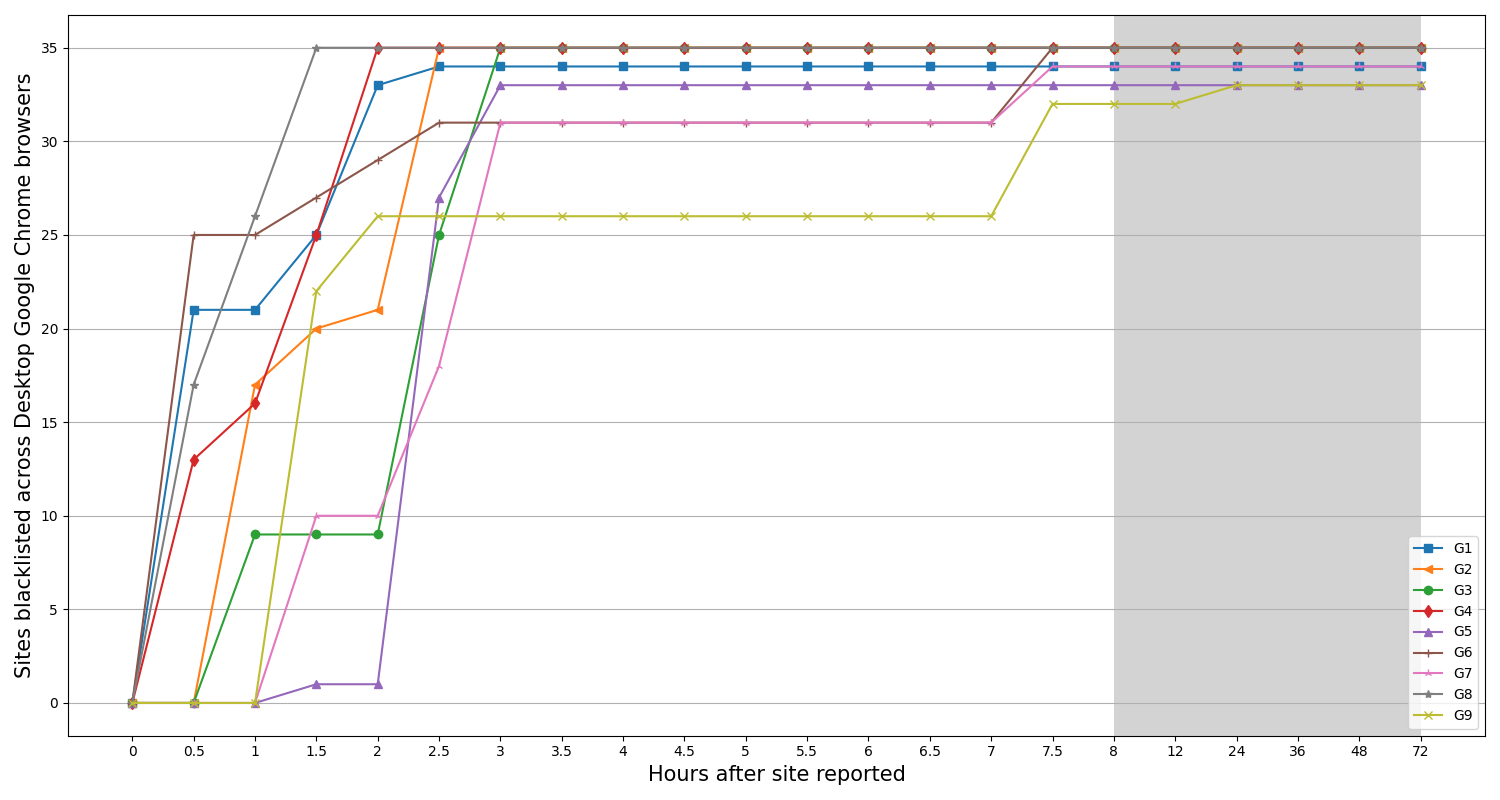
\includegraphics[width=\textwidth,height=9cm]{image (10).png}
  \caption{Desktop Blacklisting Performance}
  \label{Blacklisting speed results}
\end{figure*}

\subsection{Single-entity Reporting}

Figure \ref{Blacklisting speed results} shows blacklist coverage and speed
for reported phishing websites. In the first 30 minutes, the phishing sites with suspicious URLs, visiting from a browser with active content-based and real-time anti-phishing, and without using cloaking has most blacklisted sites. During the first three of the experiment average, 95\%  of the phishing sites became blacklist regardless of evasion method.
Our study demonstrates that reporting has the most significant role in the blacklisting of un-seen phishing sites.
%add more about content-based to discussion

\section{Discussion}
This section discusses the limitations of our work and suggestions for improving the client-side content-based anti-phishing mechanism.

Even though blacklists have the ability to detect the typical evasion techniques which are tested in our work as well as in the previous work~\cite{oest2020phishtime}, our experiments have revealed that these techniques slow the speed of the blacklisting. A significant gap also remains in blacklists' coverage on mobile devices. The client-side anti-phishing proactive approaches are defined to overcome these shortcomings.

Basically, our study's primary purpose was to evaluate client-side anti-phishing, and our experiment revealed surprising results in this regard. Although the client-side anti-phishing primary role is proactively mitigating the new phishing attacks to overcome the blacklists' delay in protecting users, for not reported websites, the client-side content-based anti-phishing does not affect blacklists coverage or speed. However, our findings show that for reported phishing websites without cloaking techniques, content-based anti-phishing accelerates blacklisting. This ecosystem suffers from serious challenges: "If client-side anti-phishing- including the content-based and real-time mechanism- does not affect the blacklisting performance, what reasons are behind deploying these methods?"

The other issue is concerning the server-side classifier. The client-side classifier sends its results to the server to make the final evaluation on the related suspicious websites; on the other hand, the real-time anti-phishing method also sends every visited URL to the server, still, this method does not affect the blacklisting. These findings raise question on the server-side classification performance or even occurrence.

Our findings could be used to improve the client-side classification accuracy. Continuous monitoring of the most recent phishing websites' structure- including URLs and the content- training the related machine-learning model, and refining the classification algorithm with this data, can further improve the client-side content-based detection.

Although the server-side classifier is not accessible, we analyze it by sending a phishing verdict for real phishing websites. During this study, we found out that the server-side classifier's results are directly proportional to the value of the client-side scorer results. Thus, our study methodology could also be used to improve the server-side classifier.

Our empirical blacklists experiment that we performed on the Chrome browser and GSB could be used to analyze other modern browsers and related entities. 
Although our work focuses on browser anti-phishing mechanism, the scope of future experiments could also be shifted to evaluate other threats( e.g, spam filters and  malware). 
% Phishing kits provides filter to avoid detecting by blacklists entities. 

\subsection{Security Recommendations}

Based on our study results, we recommend several potential improvements to Google Chrome's client-side anti-phishing ecosystem.

\textbf{Chrome client-side anti-phishing}. We believe that the highest priority within the current ecosystem should be an effective native client-side anti-phishing in both desktop and mobile browsers. The ineffectiveness of current client-side anti-phishing on blacklisting performance is sufficient for the necessity of enhancing the functionality of the client-side anti-phishing mechanisms, including content-based anti-phishing, password protection, and real-time anti-phishing. periodic performing this study could be used for evaluating this ecosystem.

\textbf{Blacklist occurrence and timeliness}. The phishing attacks' life-time is divided into two parts: the gap between the launching of phishing attacks and the detection of a phishing website and the time delay between detecting a phishing website and its blacklisting across the browsers.
Although Browser-based anti-phishing is carried on in the first part, the client-side scorer's result affects the server-side classifier result. Even though it has a greater effect on the \textit{occurrence} rather than the timeliness of blacklisting, it still affects the \textit{timeliness} of blacklisting indirectly. 

\subsection{limitations}
Even though our study revealed the Chrome browser's client-side anti-phishing ecosystem's weaknesses in the real-world, our analysis should be considered beside certain limitations.
%experimental findings

\textbf{Source Data}. Although we used an extensive sample of data of phishing websites in the blacklisting experiment, targeting a single organization(PayPal) may skew our experimental findings. 
Using the same targeted brand in our study, we just use different URL features for each phishing website. However, DOM and term features are also effective on the classifier's results. 

\textbf{Source Classifier}. To analysis chrome client-side anti-phishing, we deployed chromium source code. Since chromium is open-source and chrome is not, we didn't have access to the chrome source code. Based on the fact that the GSB anti-phishing system is not in the list of chrome's added features to chromium, we deployed chromium source code to perform our first experiment on client-side anti-phishing evaluations. 

% Our phishing websites single brand(PayPal) 
%Chromium  vs chrome 
\textbf{Reporting}. For each phishing site, we only submitted a single report, while in real-world phishing sites might encounter several automated reports from spam filters. However,  attackers can decrease the volume of phishing reports for each URL(e.g., Using redirection links).
Also, adversaries might utilize direct reports to the blacklist
operators to submit false reports or attempt to access profile crawling infrastructure.

\subsection{Disclosures}

We sent our findings in a report to Google with focus on inefficiency of client-side classifier and gaps in blacklisting on mobile devices. 
%explain the further google actions


\section{Related Work}
%%outline{
% This section will cover the following concepts:

% In the first paragraph, we mention:

% To the best of our knowledge, Our work is the first systematic measurement for client-side content-based anti-phishing in industrial browsers that provides an empirical study of the performance of client-side anti-phishing and it's effects on blacklisting rate.

% Other studies were previously done in:

% cracking Machine Learning Phishing URL classification (MLPU) system and client-side classifier model

% empirically measuring blacklists considering evasion methods

% In the second paragraph, we talk about the "Phishfarm" paper as the most similar one to our work in the term of evaluation.

% In the third and fourth paragraphs, we summarize the previous papers ( 2016 and 2019) in cracking GSB anti-phishing systems as the most similar works to our work in the term of case study as "Attacks on classifiers."

% In the fifth paragraph, we mention "Phishtime, Golden Hours and PhishTime" papers.

% In the last paragraph, we briefly mention:

% 1)so many works Phishing websites detection 2)Browsers studies 3)Comparison classifiers
%% outline}

To the best of our knowledge, Our work is the first systematic measurement for client-side content-based anti-phishing in industrial browsers that provides an empirical study of the performance of client-side anti-phishing and its effects on blacklisting rate. 

However, Other studies looking at the in-browser classifier on its own, as well as the effectiveness of the blacklisting backend, but none have evaluated the real-world effectiveness of the in-browser classifiers as they are deployed in modern browsers.
% However, other studies were previously explicitly done to crack the Machine Learning Phishing URL classification (MLPU) system and the client-side classifier model or empirically measure blacklists with and without considering evasion methods for the main browsers.

% %2016 paper:
% %Phishfarm 
The most similar work to ours is~\cite{oest2019phishfarm}. The authors have deployed a framework called ``Phishfarm" for two purposes: 

1) First, measure the timeliness of the industrial browsers' blacklist mechanism (e.g., chrome and Edge). 

2)Second, to test the effectiveness of evasion techniques against the anti-phishing ecosystem.

The authors deployed five batches of 396 fake phishing websites over two weeks using the proposed framework to measure the effectiveness of different sets of existing cloaking techniques on delaying or avoiding blacklisting in the five well known anti-phishing entities.
We adapted this framework to evaluate the effectiveness of client-side content-based and real-time anti-phishing in the main browsers.

%Machine learning approaches
%paper 2016
Liang et al.\cite{liang2016cracking} analyzed the security challenges for the client-side classifier deployed in the Chrome browser. 
The authors extracted sufficient knowledge from the client-side classifier with reverse engineering techniques. Based on the extracted information, presented a new attack to crack the client-side classifier. They successfully performed two types of evasion attacks to Google's phishing pages filter. These attacks are based on adding or removing features with considerable contributions to classifier scoring into or from the target phishing pages to decrease their phishing scores.
While this work showed that chrome's client-side classifier is vulnerable to classifiers cracking attacks, it did not consider the user's security in this ecosystem.

%paper 2019

Lei et al.\cite{lei2020advanced} carried out an evaluation on chrome's client-side classifier in 2019 and launched three types of evasion attacks on this classifier.
Uniquely, this work performed a black-box attack, an attack with no knowledge, on the chrome client-side phishing detection classifier.
The authors proposed three mutation-based attacks: (1)Black-box, (2)Grey-box, and (3)White-box. These attacks are based on the different amounts of knowledge of the target classifier. 
They presented a similarity-based method to mitigate the proposed evasion attacks. 
In addition, the authors emphasized two methods of classification rule selection to improve the robustness of the classifier.
The key difference in our work is that we not only empirically evaluate the client-side anti-phishing performance; we also assess its effect on blacklisting cover and speed in the real-world.  



% %Consequently, we found the inconsistency of blacklisting in mobile browsers, and mobile GSB browsers saw zero blacklisting after reporting to the API( anti-phishing entities). %%




%Golden Hours
Oest et al.\cite{oest2020sunrise} carried out a longitudinal end-to-end life cycle of large-scale phishing attacks to identify the gaps in detection phishing methods and achieve insight into the timing of modern phishing attacks process. The authors also measure the performance of blacklists indirectly. 
They proposed a Golden Hour framework to measure victim traffic to phishing pages and found that clusters of large attacks are significantly sophisticated.
The authors evaluated the average effect of blacklisting across the entire dataset and quantified the potential raise in victims caused by delays to emphasize the significance of sufficient blacklisting speed. This finding strengthens the importance of having efficient client-side content-based anti-phishing.

%PhishTime

%Crawl Phish

% %Phishing websites detection. so many works :
% Browsers studies
% Attacks on classifiers 
% Comparison classifiers
Earlier studies have done in blacklisting analyzing~\cite{virvilis2014mobile,abrams2013browser,sheng2009empirical}.
Other prior works have assessed the efficiency of browser security warnings against phishing attacks~\cite{akhawe2013alice,egelman2008you,dhamija2006phishing,sunshine2009crying}. Browser-based anti-phishing toolbars are widely proposed and assessed~\cite{tsalis2014browser,huang2009browser,mazher2013web,yue2008anti,marchal2017off}.
% \usepackage{multirow}
% \usepackage{colortbl}


% \usepackage{multirow}
% \usepackage{colortbl}


\section{Conclusion}

% The structure of the Conclusion part is as below:

% what we have done

% why we have done this

% why it is crucial findings
% We evaluated the protection provided by the chrome client-side anti-phishing ecosystem in the long term, with a focus on browser content-based anti-phishing. 
We performed the first long term controlled evaluation of how client-side anti-phishing defenses - including blacklists, content-based, and real-time - affect the new phishing websites' detection and blacklisting coverage and speed in the most popular web browser by launching and monitoring a large set of phishing sites. 
% The chrome browser's anti-phishing defenses - including blacklists, content-based, and real-time - are complex systems. 
َAccording to the record volume of phishing attack \cite{APWG}, these defense mechanisms detect several phishing websites. Nevertheless, Our research uncovered a significant fact that Chrome's client-side anti-phishing without reporting fails in detecting new phishing websites. In addition, our study revealed an essential inconsistency between Mobile and Desktop blacklists. 

Given the advancement of sophisticated phishing attacks, we believe that analyzing major browsers anti-phishing system is essential to identify the weaknesses, improve the browsers' defense, and protect the billions of users from attackers. In addition, our study provide clear picture of users' privacy in the browser client-side anti-phishing system.

% In the future, we will 
Analysis of data from our empirical measurement, we believe that longitudinal measurements of the modern browsers' anti-phishing ecosystem are crucial not only for maintaining a comprehension
of the modern browsers' protection, but also for
evaluating new security features as they are released to prove that the security of users can be continuously ensured.


\bibliographystyle{plain}
\bibliography{reference}

\end{document}




